\documentclass[a4paper]{report}

%%%%%%%%%%%%%%%%%%%%%%%%%%%%%%%%%
% PACKAGE IMPORTS
%%%%%%%%%%%%%%%%%%%%%%%%%%%%%%%%%


\usepackage[tmargin=2cm,rmargin=1in,lmargin=1in,margin=0.85in,bmargin=2cm,footskip=.2in]{geometry}
\usepackage[onehalfspacing]{setspace}
\usepackage{graphicx}
\usepackage{float}
% 以下包可根据需要启用
\usepackage{icomma}
\usepackage{nicematrix}
\usepackage[english]{babel}
\usepackage{csquotes}
\usepackage[T1]{fontenc} % 注意：可能与xeCJK冲突
\usepackage[locale = US,space-before-unit=true,per-mode = symbol]{siunitx}
\usepackage{placeins}
\usepackage{booktabs}
\usepackage{multirow}
\usepackage{arydshln}
\usepackage{amsmath,amsfonts,amsthm,amssymb,mathtools}
\usepackage[varbb]{newpxmath}
\usepackage{xfrac}
\usepackage{xeCJK}
\IfFontExistsTF{Source Han Serif}
    {\setCJKmainfont{Source Han Serif}}
    {\setCJKmainfont{FandolSong-Regular.otf}[BoldFont=FandolSong-Bold.otf]}
\usepackage[makeroom]{cancel}
\usepackage{mathtools}
\usepackage{bookmark}
\usepackage{enumitem}
\usepackage{hyperref,theoremref}
\hypersetup{
	pdftitle={Assignment},
	colorlinks=true, linkcolor=whusakura, urlcolor=whusakura,
	bookmarksnumbered=true,
	bookmarksopen=true
}
\usepackage[most,many,breakable]{tcolorbox}
\usepackage{xcolor}
\usepackage{varwidth}
\usepackage{varwidth}
\usepackage{etoolbox}
\usepackage{makecell}
%\usepackage{authblk}
\usepackage{nameref}
\usepackage{multicol,array}
\usepackage{tikz-cd}
\usepackage{pgfplots}
\usepgfplotslibrary{groupplots}
\usepackage[ruled,vlined,linesnumbered]{algorithm2e}
\usepackage{comment} % enables the use of multi-line comments (\ifx \fi) 
\usepackage{import}
\usepackage{xifthen}
\usepackage{pdfpages}

\newcommand\mycommfont[1]{\footnotesize\ttfamily\textcolor{blue}{#1}}
\SetCommentSty{mycommfont}
\newcommand{\incfig}[1]{%
    \def\svgwidth{\columnwidth}
    \import{./figures/}{#1.pdf_tex}
}

\usepackage{tikzsymbols}
\renewcommand\qedsymbol{$\Laughey$}


%\usepackage{import}
%\usepackage{xifthen}
%\usepackage{pdfpages}
%\usepackage{transparent}


%%%%%%%%%%%%%%%%%%%%%%%%%%%%%%
% SELF MADE COLORS
%%%%%%%%%%%%%%%%%%%%%%%%%%%%%%



\definecolor{whusakura}{RGB}{248, 163, 188}
\definecolor{myg}{RGB}{56, 140, 70}
\definecolor{myb}{RGB}{45, 111, 177}
\definecolor{myr}{RGB}{199, 68, 64}
\definecolor{mytheorembg}{HTML}{F2F2F9}
\definecolor{mytheoremfr}{HTML}{00007B}
\definecolor{mylenmabg}{HTML}{FFFAF8}
\definecolor{mylenmafr}{HTML}{983b0f}
\definecolor{mypropbg}{HTML}{f2fbfc}
\definecolor{mypropfr}{HTML}{191971}
\definecolor{myexamplebg}{HTML}{F2FBF8}
\definecolor{myexamplefr}{HTML}{88D6D1}
\definecolor{myexampleti}{HTML}{2A7F7F}
\definecolor{mydefinitbg}{HTML}{E5E5FF}
\definecolor{mydefinitfr}{HTML}{3F3FA3}
\definecolor{notesgreen}{RGB}{0,162,0}
\definecolor{myp}{RGB}{197, 92, 212}
\definecolor{mygr}{HTML}{2C3338}
\definecolor{myred}{RGB}{127,0,0}
\definecolor{myyellow}{RGB}{169,121,69}
\definecolor{myexercisebg}{HTML}{F2FBF8}
\definecolor{myexercisefg}{HTML}{88D6D1}


%%%%%%%%%%%%%%%%%%%%%%%%%%%%
% TCOLORBOX SETUPS
%%%%%%%%%%%%%%%%%%%%%%%%%%%%

\setlength{\parindent}{1cm}
%================================
% THEOREM BOX
%================================

\tcbuselibrary{theorems,skins,hooks}
\newtcbtheorem[number within=section]{Theorem}{Theorem}
{%
	enhanced,
	breakable,
	colback = mytheorembg,
	frame hidden,
	boxrule = 0sp,
	borderline west = {2pt}{0pt}{mytheoremfr},
	sharp corners,
	detach title,
	before upper = \tcbtitle\par\smallskip,
	coltitle = mytheoremfr,
	fonttitle = \bfseries\sffamily,
	description font = \mdseries,
	separator sign none,
	segmentation style={solid, mytheoremfr},
}
{th}

\tcbuselibrary{theorems,skins,hooks}
\newtcbtheorem[number within=chapter]{theorem}{Theorem}
{%
	enhanced,
	breakable,
	colback = mytheorembg,
	frame hidden,
	boxrule = 0sp,
	borderline west = {2pt}{0pt}{mytheoremfr},
	sharp corners,
	detach title,
	before upper = \tcbtitle\par\smallskip,
	coltitle = mytheoremfr,
	fonttitle = \bfseries\sffamily,
	description font = \mdseries,
	separator sign none,
	segmentation style={solid, mytheoremfr},
}
{th}


\tcbuselibrary{theorems,skins,hooks}
\newtcolorbox{Theoremcon}
{%
	enhanced
	,breakable
	,colback = mytheorembg
	,frame hidden
	,boxrule = 0sp
	,borderline west = {2pt}{0pt}{mytheoremfr}
	,sharp corners
	,description font = \mdseries
	,separator sign none
}

%================================
% Corollery
%================================
\tcbuselibrary{theorems,skins,hooks}
\newtcbtheorem[number within=section]{Corollary}{Corollary}
{%
	enhanced
	,breakable
	,colback = myp!10
	,frame hidden
	,boxrule = 0sp
	,borderline west = {2pt}{0pt}{myp!85!black}
	,sharp corners
	,detach title
	,before upper = \tcbtitle\par\smallskip
	,coltitle = myp!85!black
	,fonttitle = \bfseries\sffamily
	,description font = \mdseries
	,separator sign none
	,segmentation style={solid, myp!85!black}
}
{th}
\tcbuselibrary{theorems,skins,hooks}
\newtcbtheorem[number within=chapter]{corollary}{Corollary}
{%
	enhanced
	,breakable
	,colback = myp!10
	,frame hidden
	,boxrule = 0sp
	,borderline west = {2pt}{0pt}{myp!85!black}
	,sharp corners
	,detach title
	,before upper = \tcbtitle\par\smallskip
	,coltitle = myp!85!black
	,fonttitle = \bfseries\sffamily
	,description font = \mdseries
	,separator sign none
	,segmentation style={solid, myp!85!black}
}
{th}


%================================
% LENMA
%================================

\tcbuselibrary{theorems,skins,hooks}
\newtcbtheorem[number within=section]{Lenma}{Lenma}
{%
	enhanced,
	breakable,
	colback = mylenmabg,
	frame hidden,
	boxrule = 0sp,
	borderline west = {2pt}{0pt}{mylenmafr},
	sharp corners,
	detach title,
	before upper = \tcbtitle\par\smallskip,
	coltitle = mylenmafr,
	fonttitle = \bfseries\sffamily,
	description font = \mdseries,
	separator sign none,
	segmentation style={solid, mylenmafr},
}
{th}

\tcbuselibrary{theorems,skins,hooks}
\newtcbtheorem[number within=chapter]{lenma}{Lenma}
{%
	enhanced,
	breakable,
	colback = mylenmabg,
	frame hidden,
	boxrule = 0sp,
	borderline west = {2pt}{0pt}{mylenmafr},
	sharp corners,
	detach title,
	before upper = \tcbtitle\par\smallskip,
	coltitle = mylenmafr,
	fonttitle = \bfseries\sffamily,
	description font = \mdseries,
	separator sign none,
	segmentation style={solid, mylenmafr},
}
{th}


%================================
% PROPOSITION
%================================

\tcbuselibrary{theorems,skins,hooks}
\newtcbtheorem[number within=section]{Prop}{Proposition}
{%
	enhanced,
	breakable,
	colback = mypropbg,
	frame hidden,
	boxrule = 0sp,
	borderline west = {2pt}{0pt}{mypropfr},
	sharp corners,
	detach title,
	before upper = \tcbtitle\par\smallskip,
	coltitle = mypropfr,
	fonttitle = \bfseries\sffamily,
	description font = \mdseries,
	separator sign none,
	segmentation style={solid, mypropfr},
}
{th}

\tcbuselibrary{theorems,skins,hooks}
\newtcbtheorem[number within=chapter]{prop}{Proposition}
{%
	enhanced,
	breakable,
	colback = mypropbg,
	frame hidden,
	boxrule = 0sp,
	borderline west = {2pt}{0pt}{mypropfr},
	sharp corners,
	detach title,
	before upper = \tcbtitle\par\smallskip,
	coltitle = mypropfr,
	fonttitle = \bfseries\sffamily,
	description font = \mdseries,
	separator sign none,
	segmentation style={solid, mypropfr},
}
{th}


%================================
% CLAIM
%================================

\tcbuselibrary{theorems,skins,hooks}
\newtcbtheorem[number within=section]{claim}{Claim}
{%
	enhanced
	,breakable
	,colback = myg!10
	,frame hidden
	,boxrule = 0sp
	,borderline west = {2pt}{0pt}{myg}
	,sharp corners
	,detach title
	,before upper = \tcbtitle\par\smallskip
	,coltitle = myg!85!black
	,fonttitle = \bfseries\sffamily
	,description font = \mdseries
	,separator sign none
	,segmentation style={solid, myg!85!black}
}
{th}



%================================
% Exercise
%================================

\tcbuselibrary{theorems,skins,hooks}
\newtcbtheorem[number within=section]{Exercise}{Exercise}
{%
	enhanced,
	breakable,
	colback = myexercisebg,
	frame hidden,
	boxrule = 0sp,
	borderline west = {2pt}{0pt}{myexercisefg},
	sharp corners,
	detach title,
	before upper = \tcbtitle\par\smallskip,
	coltitle = myexercisefg,
	fonttitle = \bfseries\sffamily,
	description font = \mdseries,
	separator sign none,
	segmentation style={solid, myexercisefg},
}
{th}

\tcbuselibrary{theorems,skins,hooks}
\newtcbtheorem[number within=chapter]{exercise}{Exercise}
{%
	enhanced,
	breakable,
	colback = myexercisebg,
	frame hidden,
	boxrule = 0sp,
	borderline west = {2pt}{0pt}{myexercisefg},
	sharp corners,
	detach title,
	before upper = \tcbtitle\par\smallskip,
	coltitle = myexercisefg,
	fonttitle = \bfseries\sffamily,
	description font = \mdseries,
	separator sign none,
	segmentation style={solid, myexercisefg},
}
{th}

%================================
% EXAMPLE BOX
%================================

\newtcbtheorem[number within=section]{Example}{Example}
{%
	colback = myexamplebg
	,breakable
	,colframe = myexamplefr
	,coltitle = myexampleti
	,boxrule = 1pt
	,sharp corners
	,detach title
	,before upper=\tcbtitle\par\smallskip
	,fonttitle = \bfseries
	,description font = \mdseries
	,separator sign none
	,description delimiters parenthesis
}
{ex}

\newtcbtheorem[number within=chapter]{example}{Example}
{%
	colback = myexamplebg
	,breakable
	,colframe = myexamplefr
	,coltitle = myexampleti
	,boxrule = 1pt
	,sharp corners
	,detach title
	,before upper=\tcbtitle\par\smallskip
	,fonttitle = \bfseries
	,description font = \mdseries
	,separator sign none
	,description delimiters parenthesis
}
{ex}

%================================
% DEFINITION BOX
%================================

\newtcbtheorem[number within=section]{Definition}{Definition}{enhanced,
	before skip=2mm,after skip=2mm, colback=red!5,colframe=red!80!black,boxrule=0.5mm,
	attach boxed title to top left={xshift=1cm,yshift*=1mm-\tcboxedtitleheight}, varwidth boxed title*=-3cm,
	boxed title style={frame code={
					\path[fill=tcbcolback]
					([yshift=-1mm,xshift=-1mm]frame.north west)
					arc[start angle=0,end angle=180,radius=1mm]
					([yshift=-1mm,xshift=1mm]frame.north east)
					arc[start angle=180,end angle=0,radius=1mm];
					\path[left color=tcbcolback!60!black,right color=tcbcolback!60!black,
						middle color=tcbcolback!80!black]
					([xshift=-2mm]frame.north west) -- ([xshift=2mm]frame.north east)
					[rounded corners=1mm]-- ([xshift=1mm,yshift=-1mm]frame.north east)
					-- (frame.south east) -- (frame.south west)
					-- ([xshift=-1mm,yshift=-1mm]frame.north west)
					[sharp corners]-- cycle;
				},interior engine=empty,
		},
	fonttitle=\bfseries,
	title={#2},#1}{def}
\newtcbtheorem[number within=chapter]{definition}{Definition}{enhanced,
	before skip=2mm,after skip=2mm, colback=red!5,colframe=red!80!black,boxrule=0.5mm,
	attach boxed title to top left={xshift=1cm,yshift*=1mm-\tcboxedtitleheight}, varwidth boxed title*=-3cm,
	boxed title style={frame code={
					\path[fill=tcbcolback]
					([yshift=-1mm,xshift=-1mm]frame.north west)
					arc[start angle=0,end angle=180,radius=1mm]
					([yshift=-1mm,xshift=1mm]frame.north east)
					arc[start angle=180,end angle=0,radius=1mm];
					\path[left color=tcbcolback!60!black,right color=tcbcolback!60!black,
						middle color=tcbcolback!80!black]
					([xshift=-2mm]frame.north west) -- ([xshift=2mm]frame.north east)
					[rounded corners=1mm]-- ([xshift=1mm,yshift=-1mm]frame.north east)
					-- (frame.south east) -- (frame.south west)
					-- ([xshift=-1mm,yshift=-1mm]frame.north west)
					[sharp corners]-- cycle;
				},interior engine=empty,
		},
	fonttitle=\bfseries,
	title={#2},#1}{def}



%================================
% Solution BOX
%================================

\makeatletter
\newtcbtheorem{question}{Question}{enhanced,
	breakable,
	colback=white,
	colframe=myb!80!black,
	attach boxed title to top left={yshift*=-\tcboxedtitleheight},
	fonttitle=\bfseries,
	title={#2},
	boxed title size=title,
	boxed title style={%
			sharp corners,
			rounded corners=northwest,
			colback=tcbcolframe,
			boxrule=0pt,
		},
	underlay boxed title={%
			\path[fill=tcbcolframe] (title.south west)--(title.south east)
			to[out=0, in=180] ([xshift=5mm]title.east)--
			(title.center-|frame.east)
			[rounded corners=\kvtcb@arc] |-
			(frame.north) -| cycle;
		},
	#1
}{def}
\makeatother

%================================
% SOLUTION BOX
%================================

\makeatletter
\newtcolorbox{solution}{enhanced,
	breakable,
	colback=white,
	colframe=myg!80!black,
	attach boxed title to top left={yshift*=-\tcboxedtitleheight},
	title=Solution,
	boxed title size=title,
	boxed title style={%
			sharp corners,
			rounded corners=northwest,
			colback=tcbcolframe,
			boxrule=0pt,
		},
	underlay boxed title={%
			\path[fill=tcbcolframe] (title.south west)--(title.south east)
			to[out=0, in=180] ([xshift=5mm]title.east)--
			(title.center-|frame.east)
			[rounded corners=\kvtcb@arc] |-
			(frame.north) -| cycle;
		},
}
\makeatother

%================================
% Question BOX
%================================

\makeatletter
\newtcbtheorem{qstion}{Question}{enhanced,
	breakable,
	colback=white,
	colframe=mygr,
	attach boxed title to top left={yshift*=-\tcboxedtitleheight},
	fonttitle=\bfseries,
	title={#2},
	boxed title size=title,
	boxed title style={%
			sharp corners,
			rounded corners=northwest,
			colback=tcbcolframe,
			boxrule=0pt,
		},
	underlay boxed title={%
			\path[fill=tcbcolframe] (title.south west)--(title.south east)
			to[out=0, in=180] ([xshift=5mm]title.east)--
			(title.center-|frame.east)
			[rounded corners=\kvtcb@arc] |-
			(frame.north) -| cycle;
		},
	#1
}{def}
\makeatother

\newtcbtheorem[number within=chapter]{wconc}{Wrong Concept}{
	breakable,
	enhanced,
	colback=white,
	colframe=myr,
	arc=0pt,
	outer arc=0pt,
	fonttitle=\bfseries\sffamily\large,
	colbacktitle=myr,
	attach boxed title to top left={},
	boxed title style={
			enhanced,
			skin=enhancedfirst jigsaw,
			arc=3pt,
			bottom=0pt,
			interior style={fill=myr}
		},
	#1
}{def}



%================================
% NOTE BOX
%================================

\usetikzlibrary{backgrounds, 3d, arrows, calc, quotes, shadows.blur, arrows.meta, decorations.pathreplacing, decorations.markings}
\usetikzlibrary{tikzmark, fit, shapes.geometric, positioning, shapes.arrows, patterns}
\tcbuselibrary{skins}
\newtcolorbox{note}[1][]{%
	enhanced jigsaw,
	colback=gray!20!white,%
	colframe=gray!80!black,
	size=small,
	boxrule=1pt,
	title=\textbf{Note:-},
	halign title=flush center,
	coltitle=black,
	breakable,
	drop shadow=black!50!white,
	attach boxed title to top left={xshift=1cm,yshift=-\tcboxedtitleheight/2,yshifttext=-\tcboxedtitleheight/2},
	minipage boxed title=1.5cm,
	boxed title style={%
			colback=white,
			size=fbox,
			boxrule=1pt,
			boxsep=2pt,
			underlay={%
					\coordinate (dotA) at ($(interior.west) + (-0.5pt,0)$);
					\coordinate (dotB) at ($(interior.east) + (0.5pt,0)$);
					\begin{scope}
						\clip (interior.north west) rectangle ([xshift=3ex]interior.east);
						\filldraw [white, blur shadow={shadow opacity=60, shadow yshift=-.75ex}, rounded corners=2pt] (interior.north west) rectangle (interior.south east);
					\end{scope}
					\begin{scope}[gray!80!black]
						\fill (dotA) circle (2pt);
						\fill (dotB) circle (2pt);
					\end{scope}
				},
		},
	#1,
}

%%%%%%%%%%%%%%%%%%%%%%%%%%%%%%
% SELF MADE COMMANDS
%%%%%%%%%%%%%%%%%%%%%%%%%%%%%%


\newcommand{\thm}[2]{\begin{Theorem}{#1}{}#2\end{Theorem}}
\newcommand{\cor}[2]{\begin{Corollary}{#1}{}#2\end{Corollary}}
\newcommand{\mlenma}[2]{\begin{Lenma}{#1}{}#2\end{Lenma}}
\newcommand{\mprop}[2]{\begin{Prop}{#1}{}#2\end{Prop}}
\newcommand{\clm}[3]{\begin{claim}{#1}{#2}#3\end{claim}}
\newcommand{\wc}[2]{\begin{wconc}{#1}{}\setlength{\parindent}{1cm}#2\end{wconc}}
\newcommand{\thmcon}[1]{\begin{Theoremcon}{#1}\end{Theoremcon}}
\newcommand{\ex}[2]{\begin{Example}{#1}{}#2\end{Example}}
\newcommand{\dfn}[2]{\begin{Definition}[colbacktitle=red!75!black]{#1}{}#2\end{Definition}}
\newcommand{\dfnc}[2]{\begin{definition}[colbacktitle=red!75!black]{#1}{}#2\end{definition}}
\newcommand{\qs}[2]{\begin{question}{#1}{}#2\end{question}}
\newcommand{\pf}[2]{\begin{myproof}[#1]#2\end{myproof}}
\newcommand{\nt}[1]{\begin{note}#1\end{note}}

\newcommand*\circled[1]{\tikz[baseline=(char.base)]{
		\node[shape=circle,draw,inner sep=1pt] (char) {#1};}}
\newcommand\getcurrentref[1]{%
	\ifnumequal{\value{#1}}{0}
	{??}
	{\the\value{#1}}%
}
\newcommand{\getCurrentSectionNumber}{\getcurrentref{section}}
\newenvironment{myproof}[1][\proofname]{%
	\proof[\bfseries #1: ]%
}{\endproof}

\newcommand{\mclm}[2]{\begin{myclaim}[#1]#2\end{myclaim}}
\newenvironment{myclaim}[1][\claimname]{\proof[\bfseries #1: ]}{}

\newcounter{mylabelcounter}

\makeatletter
\newcommand{\setword}[2]{%
	\phantomsection
	#1\def\@currentlabel{\unexpanded{#1}}\label{#2}%
}
\makeatother




\tikzset{
	symbol/.style={
			draw=none,
			every to/.append style={
					edge node={node [sloped, allow upside down, auto=false]{$#1$}}}
		}
}


% deliminators
\DeclarePairedDelimiter{\abs}{\lvert}{\rvert}
\DeclarePairedDelimiter{\norm}{\lVert}{\rVert}

\DeclarePairedDelimiter{\ceil}{\lceil}{\rceil}
\DeclarePairedDelimiter{\floor}{\lfloor}{\rfloor}
\DeclarePairedDelimiter{\round}{\lfloor}{\rceil}

\newsavebox\diffdbox
\newcommand{\slantedromand}{{\mathpalette\makesl{d}}}
\newcommand{\makesl}[2]{%
\begingroup
\sbox{\diffdbox}{$\mathsurround=0pt#1\mathrm{#2}$}%
\pdfsave
\pdfsetmatrix{1 0 0.2 1}%
\rlap{\usebox{\diffdbox}}%
\pdfrestore
\hskip\wd\diffdbox
\endgroup
}
\newcommand{\dd}[1][]{\ensuremath{\mathop{}\!\ifstrempty{#1}{%
\slantedromand\@ifnextchar^{\hspace{0.2ex}}{\hspace{0.1ex}}}%
{\slantedromand\hspace{0.2ex}^{#1}}}}
\ProvideDocumentCommand\dv{o m g}{%
  \ensuremath{%
    \IfValueTF{#3}{%
      \IfNoValueTF{#1}{%
        \frac{\dd #2}{\dd #3}%
      }{%
        \frac{\dd^{#1} #2}{\dd #3^{#1}}%
      }%
    }{%
      \IfNoValueTF{#1}{%
        \frac{\dd}{\dd #2}%
      }{%
        \frac{\dd^{#1}}{\dd #2^{#1}}%
      }%
    }%
  }%
}
\providecommand*{\pdv}[3][]{\frac{\partial^{#1}#2}{\partial#3^{#1}}}
%  - others
\DeclareMathOperator{\Lap}{\mathcal{L}}
\DeclareMathOperator{\Var}{Var} % varience
\DeclareMathOperator{\Cov}{Cov} % covarience
\DeclareMathOperator{\E}{E} % expected

% Since the amsthm package isn't loaded

% I prefer the slanted \leq
\let\oldleq\leq % save them in case they're every wanted
\let\oldgeq\geq
\renewcommand{\leq}{\leqslant}
\renewcommand{\geq}{\geqslant}

% % redefine matrix env to allow for alignment, use r as default
% \renewcommand*\env@matrix[1][r]{\hskip -\arraycolsep
%     \let\@ifnextchar\new@ifnextchar
%     \array{*\c@MaxMatrixCols #1}}


%\usepackage{framed}
%\usepackage{titletoc}
%\usepackage{etoolbox}
%\usepackage{lmodern}


%\patchcmd{\tableofcontents}{\contentsname}{\sffamily\contentsname}{}{}

%\renewenvironment{leftbar}
%{\def\FrameCommand{\hspace{6em}%
%		{\color{myyellow}\vrule width 2pt depth 6pt}\hspace{1em}}%
%	\MakeFramed{\parshape 1 0cm \dimexpr\textwidth-6em\relax\FrameRestore}\vskip2pt%
%}
%{\endMakeFramed}

%\titlecontents{chapter}
%[0em]{\vspace*{2\baselineskip}}
%{\parbox{4.5em}{%
%		\hfill\Huge\sffamily\bfseries\color{myred}\thecontentspage}%
%	\vspace*{-2.3\baselineskip}\leftbar\textsc{\small\chaptername~\thecontentslabel}\\\sffamily}
%{}{\endleftbar}
%\titlecontents{section}
%[8.4em]
%{\sffamily\contentslabel{3em}}{}{}
%{\hspace{0.5em}\nobreak\itshape\color{myred}\contentspage}
%\titlecontents{subsection}
%[8.4em]
%{\sffamily\contentslabel{3em}}{}{}  
%{\hspace{0.5em}\nobreak\itshape\color{myred}\contentspage}



%%%%%%%%%%%%%%%%%%%%%%%%%%%%%%%%%%%%%%%%%%%
% TABLE OF CONTENTS
%%%%%%%%%%%%%%%%%%%%%%%%%%%%%%%%%%%%%%%%%%%

\usepackage{tikz}
\usepackage{titletoc}
\contentsmargin{0cm}
\titlecontents{chapter}[3.7pc]
{\addvspace{30pt}%
	\begin{tikzpicture}[remember picture, overlay]%
		\draw[fill=whusakura,draw=whusakura] (-7,-.1) rectangle (-0.9,.5);%
		\pgftext[left,x=-3.5cm,y=0.2cm]{\color{white}\Large\sc\bfseries Chapter\ \thecontentslabel}%
	\end{tikzpicture}\color{whusakura}\large\sc\bfseries}%
{}
{}
{\;\titlerule\;\large\sc\bfseries Page \thecontentspage
	\begin{tikzpicture}[remember picture, overlay]
		\draw[fill=whusakura,draw=whusakura] (2pt,0) rectangle (4,0.1pt);
	\end{tikzpicture}}%
\titlecontents{section}[3.7pc]
{\addvspace{2pt}}
{\contentslabel[\thecontentslabel]{2pc}}
{}
{\hfill\small \thecontentspage}
[]

% subsections 显示在同一行（紧凑格式）
\titlecontents*{subsection}[3.7pc]
{\addvspace{-1pt}\small}
{}
{}
{\ --- \small\thecontentspage}
[ \textbullet\ ][]

% 完全禁用 subsubsection：设置为空格式
%\titlecontents{subsubsection}[3.7pc]
%{} % 间距为空
%{} % 标签为空
%{} % 标题为空
%{} % 引导线为空
%{} % 页码为空

\makeatletter
% 让 LaTeX 在读取 .toc 文件时忽略 subsubsection 条目
\renewcommand{\l@subsubsection}{\@gobbletwo}
\renewcommand{\tableofcontents}{%
	\chapter*{%
	  \vspace*{-20\p@}%
	  \begin{tikzpicture}[remember picture, overlay]%
	  \pgftext[right,x=15cm,y=0.2cm]{\color{whusakura}\Huge\sc\bfseries \contentsname}%
		  \draw[fill=whusakura,draw=whusakura] (13,-.75) rectangle (20,1);%
		  \clip (13,-.75) rectangle (20,1);
	  \pgftext[right,x=15cm,y=0.2cm]{\color{white}\Huge\sc\bfseries \contentsname}%
	  \end{tikzpicture}}%
	\@starttoc{toc}}
\makeatother



%%%% 添加的包 %%%%

%From M275 "Topology" at SJSU
\newcommand{\id}{\mathrm{id}}
\newcommand{\taking}[1]{\xrightarrow{#1}}
\newcommand{\inv}{^{-1}}

%From M170 "Introduction to Graph Theory" at SJSU
\DeclareMathOperator{\diam}{diam}
\DeclareMathOperator{\ord}{ord}
\newcommand{\defeq}{\overset{\mathrm{def}}{=}}

%From the USAMO .tex files
\newcommand{\ts}{\textsuperscript}
\newcommand{\dg}{^\circ}
\newcommand{\ii}{\item}

% % From Math 55 and Math 145 at Harvard
% \newenvironment{subproof}[1][Proof]{%
% \begin{proof}[#1] \renewcommand{\qedsymbol}{$\blacksquare$}}%
% {\end{proof}}

\newcommand{\liff}{\leftrightarrow}
\newcommand{\lthen}{\rightarrow}
\newcommand{\opname}{\operatorname}
\newcommand{\surjto}{\twoheadrightarrow}
\newcommand{\injto}{\hookrightarrow}
\newcommand{\On}{\mathrm{On}} % ordinals
\DeclareMathOperator{\img}{im} % Image
\DeclareMathOperator{\Img}{Im} % Image
\DeclareMathOperator{\coker}{coker} % Cokernel
\DeclareMathOperator{\Coker}{Coker} % Cokernel
\DeclareMathOperator{\Ker}{Ker} % Kernel
\DeclareMathOperator{\rank}{rank}
\DeclareMathOperator{\Spec}{Spec} % spectrum
\DeclareMathOperator{\Tr}{Tr} % trace
\DeclareMathOperator{\pr}{pr} % projection
\DeclareMathOperator{\ext}{ext} % extension
\DeclareMathOperator{\pred}{pred} % predecessor
\DeclareMathOperator{\dom}{dom} % domain
\DeclareMathOperator{\ran}{ran} % range
\DeclareMathOperator{\Hom}{Hom} % homomorphism
\DeclareMathOperator{\Mor}{Mor} % morphisms
\DeclareMathOperator{\End}{End} % endomorphism

\newcommand{\eps}{\epsilon}
\newcommand{\veps}{\varepsilon}
\newcommand{\ol}{\overline}
\newcommand{\ul}{\underline}
\newcommand{\wt}{\widetilde}
\newcommand{\wh}{\widehat}
\newcommand{\vocab}[1]{\textbf{\color{blue} #1}}
\providecommand{\half}{\frac{1}{2}}
\newcommand{\dang}{\measuredangle} %% Directed angle
\newcommand{\ray}[1]{\overrightarrow{#1}}
\newcommand{\seg}[1]{\overline{#1}}
\newcommand{\arc}[1]{\wideparen{#1}}
\DeclareMathOperator{\cis}{cis}
\DeclareMathOperator*{\lcm}{lcm}
\DeclareMathOperator*{\argmin}{arg min}
\DeclareMathOperator*{\argmax}{arg max}
\newcommand{\cycsum}{\sum_{\mathrm{cyc}}}
\newcommand{\symsum}{\sum_{\mathrm{sym}}}
\newcommand{\cycprod}{\prod_{\mathrm{cyc}}}
\newcommand{\symprod}{\prod_{\mathrm{sym}}}
\newcommand{\Qed}{\begin{flushright}\qed\end{flushright}}
\newcommand{\parinn}{\setlength{\parindent}{1cm}}
\newcommand{\parinf}{\setlength{\parindent}{0cm}}
% \newcommand{\norm}{\|\cdot\|}
\newcommand{\inorm}{\norm_{\infty}}
\newcommand{\opensets}{\{V_{\alpha}\}_{\alpha\in I}}
\newcommand{\oset}{V_{\alpha}}
\newcommand{\opset}[1]{V_{\alpha_{#1}}}
\newcommand{\lub}{\text{lub}}
\newcommand{\del}[2]{\frac{\partial #1}{\partial #2}}
\newcommand{\Del}[3]{\frac{\partial^{#1} #2}{\partial^{#1} #3}}
\newcommand{\deld}[2]{\dfrac{\partial #1}{\partial #2}}
\newcommand{\Deld}[3]{\dfrac{\partial^{#1} #2}{\partial^{#1} #3}}
\newcommand{\lm}{\lambda}
\newcommand{\uin}{\mathbin{\rotatebox[origin=c]{90}{$\in$}}}
\newcommand{\usubset}{\mathbin{\rotatebox[origin=c]{90}{$\subset$}}}
\newcommand{\lt}{\left}
\newcommand{\rt}{\right}
\newcommand{\bs}[1]{\boldsymbol{#1}}
\newcommand{\exs}{\exists}
\newcommand{\st}{\strut}
\newcommand{\dps}[1]{\displaystyle{#1}}

\newcommand{\sol}{\setlength{\parindent}{0cm}\textbf{\textit{Solution:}}\setlength{\parindent}{1cm} }
\newcommand{\solve}[1]{\setlength{\parindent}{0cm}\textbf{\textit{Solution: }}\setlength{\parindent}{1cm}#1 \Qed}

% Things Lie
% Things Lie
\newcommand{\kb}{\mathfrak b}
\newcommand{\kg}{\mathfrak g}
\newcommand{\kh}{\mathfrak h}
\newcommand{\kn}{\mathfrak n}
\newcommand{\ku}{\mathfrak u}
\newcommand{\kz}{\mathfrak z}
\DeclareMathOperator{\Ext}{Ext} % Ext functor
\DeclareMathOperator{\Tor}{Tor} % Tor functor
\newcommand{\gl}{\opname{\mathfrak{gl}}} % frak gl group
\renewcommand{\sl}{\opname{\mathfrak{sl}}} % frak sl group chktex 6

% More script letters etc.
\newcommand{\SA}{\mathcal A}
\newcommand{\SB}{\mathcal B}
\newcommand{\SC}{\mathcal C}
\newcommand{\SF}{\mathcal F}
\newcommand{\SG}{\mathcal G}
\newcommand{\SH}{\mathcal H}
\newcommand{\OO}{\mathcal O}

\newcommand{\SCA}{\mathscr A}
\newcommand{\SCB}{\mathscr B}
\newcommand{\SCC}{\mathscr C}
\newcommand{\SCD}{\mathscr D}
\newcommand{\SCE}{\mathscr E}
\newcommand{\SCF}{\mathscr F}
\newcommand{\SCG}{\mathscr G}
\newcommand{\SCH}{\mathscr H}

% Mathfrak primes
\newcommand{\km}{\mathfrak m}
\newcommand{\kp}{\mathfrak p}
\newcommand{\kq}{\mathfrak q}

% number sets
\newcommand{\RR}[1][]{\ensuremath{\ifstrempty{#1}{\mathbb{R}}{\mathbb{R}^{#1}}}}
\newcommand{\NN}[1][]{\ensuremath{\ifstrempty{#1}{\mathbb{N}}{\mathbb{N}^{#1}}}}
\newcommand{\ZZ}[1][]{\ensuremath{\ifstrempty{#1}{\mathbb{Z}}{\mathbb{Z}^{#1}}}}
\newcommand{\QQ}[1][]{\ensuremath{\ifstrempty{#1}{\mathbb{Q}}{\mathbb{Q}^{#1}}}}
\newcommand{\CC}[1][]{\ensuremath{\ifstrempty{#1}{\mathbb{C}}{\mathbb{C}^{#1}}}}
\newcommand{\PP}[1][]{\ensuremath{\ifstrempty{#1}{\mathbb{P}}{\mathbb{P}^{#1}}}}
\newcommand{\HH}[1][]{\ensuremath{\ifstrempty{#1}{\mathbb{H}}{\mathbb{H}^{#1}}}}
\newcommand{\FF}[1][]{\ensuremath{\ifstrempty{#1}{\mathbb{F}}{\mathbb{F}^{#1}}}}
% expected value
\newcommand{\EE}{\ensuremath{\mathbb{E}}}
\newcommand{\charin}{\text{ char }}
\DeclareMathOperator{\sign}{sign}
\DeclareMathOperator{\Aut}{Aut}
\DeclareMathOperator{\Inn}{Inn}
\DeclareMathOperator{\Syl}{Syl}
\DeclareMathOperator{\Gal}{Gal}
\DeclareMathOperator{\GL}{GL} % General linear group
\DeclareMathOperator{\SL}{SL} % Special linear group

%---------------------------------------
% BlackBoard Math Fonts :-
%---------------------------------------

%Captital Letters
\newcommand{\bbA}{\mathbb{A}}	\newcommand{\bbB}{\mathbb{B}}
\newcommand{\bbC}{\mathbb{C}}	\newcommand{\bbD}{\mathbb{D}}
\newcommand{\bbE}{\mathbb{E}}	\newcommand{\bbF}{\mathbb{F}}
\newcommand{\bbG}{\mathbb{G}}	\newcommand{\bbH}{\mathbb{H}}
\newcommand{\bbI}{\mathbb{I}}	\newcommand{\bbJ}{\mathbb{J}}
\newcommand{\bbK}{\mathbb{K}}	\newcommand{\bbL}{\mathbb{L}}
\newcommand{\bbM}{\mathbb{M}}	\newcommand{\bbN}{\mathbb{N}}
\newcommand{\bbO}{\mathbb{O}}	\newcommand{\bbP}{\mathbb{P}}
\newcommand{\bbQ}{\mathbb{Q}}	\newcommand{\bbR}{\mathbb{R}}
\newcommand{\bbS}{\mathbb{S}}	\newcommand{\bbT}{\mathbb{T}}
\newcommand{\bbU}{\mathbb{U}}	\newcommand{\bbV}{\mathbb{V}}
\newcommand{\bbW}{\mathbb{W}}	\newcommand{\bbX}{\mathbb{X}}
\newcommand{\bbY}{\mathbb{Y}}	\newcommand{\bbZ}{\mathbb{Z}}

%---------------------------------------
% MathCal Fonts :-
%---------------------------------------

%Captital Letters
\newcommand{\mcA}{\mathcal{A}}	\newcommand{\mcB}{\mathcal{B}}
\newcommand{\mcC}{\mathcal{C}}	\newcommand{\mcD}{\mathcal{D}}
\newcommand{\mcE}{\mathcal{E}}	\newcommand{\mcF}{\mathcal{F}}
\newcommand{\mcG}{\mathcal{G}}	\newcommand{\mcH}{\mathcal{H}}
\newcommand{\mcI}{\mathcal{I}}	\newcommand{\mcJ}{\mathcal{J}}
\newcommand{\mcK}{\mathcal{K}}	\newcommand{\mcL}{\mathcal{L}}
\newcommand{\mcM}{\mathcal{M}}	\newcommand{\mcN}{\mathcal{N}}
\newcommand{\mcO}{\mathcal{O}}	\newcommand{\mcP}{\mathcal{P}}
\newcommand{\mcQ}{\mathcal{Q}}	\newcommand{\mcR}{\mathcal{R}}
\newcommand{\mcS}{\mathcal{S}}	\newcommand{\mcT}{\mathcal{T}}
\newcommand{\mcU}{\mathcal{U}}	\newcommand{\mcV}{\mathcal{V}}
\newcommand{\mcW}{\mathcal{W}}	\newcommand{\mcX}{\mathcal{X}}
\newcommand{\mcY}{\mathcal{Y}}	\newcommand{\mcZ}{\mathcal{Z}}


%---------------------------------------
% Bold Math Fonts :-
%---------------------------------------

%Captital Letters
\newcommand{\bmA}{\boldsymbol{A}}	\newcommand{\bmB}{\boldsymbol{B}}
\newcommand{\bmC}{\boldsymbol{C}}	\newcommand{\bmD}{\boldsymbol{D}}
\newcommand{\bmE}{\boldsymbol{E}}	\newcommand{\bmF}{\boldsymbol{F}}
\newcommand{\bmG}{\boldsymbol{G}}	\newcommand{\bmH}{\boldsymbol{H}}
\newcommand{\bmI}{\boldsymbol{I}}	\newcommand{\bmJ}{\boldsymbol{J}}
\newcommand{\bmK}{\boldsymbol{K}}	\newcommand{\bmL}{\boldsymbol{L}}
\newcommand{\bmM}{\boldsymbol{M}}	\newcommand{\bmN}{\boldsymbol{N}}
\newcommand{\bmO}{\boldsymbol{O}}	\newcommand{\bmP}{\boldsymbol{P}}
\newcommand{\bmQ}{\boldsymbol{Q}}	\newcommand{\bmR}{\boldsymbol{R}}
\newcommand{\bmS}{\boldsymbol{S}}	\newcommand{\bmT}{\boldsymbol{T}}
\newcommand{\bmU}{\boldsymbol{U}}	\newcommand{\bmV}{\boldsymbol{V}}
\newcommand{\bmW}{\boldsymbol{W}}	\newcommand{\bmX}{\boldsymbol{X}}
\newcommand{\bmY}{\boldsymbol{Y}}	\newcommand{\bmZ}{\boldsymbol{Z}}
%Small Letters
\newcommand{\bma}{\boldsymbol{a}}	\newcommand{\bmb}{\boldsymbol{b}}
\newcommand{\bmc}{\boldsymbol{c}}	\newcommand{\bmd}{\boldsymbol{d}}
\newcommand{\bme}{\boldsymbol{e}}	\newcommand{\bmf}{\boldsymbol{f}}
\newcommand{\bmg}{\boldsymbol{g}}	\newcommand{\bmh}{\boldsymbol{h}}
\newcommand{\bmi}{\boldsymbol{i}}	\newcommand{\bmj}{\boldsymbol{j}}
\newcommand{\bmk}{\boldsymbol{k}}	\newcommand{\bml}{\boldsymbol{l}}
\newcommand{\bmm}{\boldsymbol{m}}	\newcommand{\bmn}{\boldsymbol{n}}
\newcommand{\bmo}{\boldsymbol{o}}	\newcommand{\bmp}{\boldsymbol{p}}
\newcommand{\bmq}{\boldsymbol{q}}	\newcommand{\bmr}{\boldsymbol{r}}
\newcommand{\bms}{\boldsymbol{s}}	\newcommand{\bmt}{\boldsymbol{t}}
\newcommand{\bmu}{\boldsymbol{u}}	\newcommand{\bmv}{\boldsymbol{v}}
\newcommand{\bmw}{\boldsymbol{w}}	\newcommand{\bmx}{\boldsymbol{x}}
\newcommand{\bmy}{\boldsymbol{y}}	\newcommand{\bmz}{\boldsymbol{z}}

%---------------------------------------
% Scr Math Fonts :-
%---------------------------------------

\newcommand{\sA}{{\mathscr{A}}}   \newcommand{\sB}{{\mathscr{B}}}
\newcommand{\sC}{{\mathscr{C}}}   \newcommand{\sD}{{\mathscr{D}}}
\newcommand{\sE}{{\mathscr{E}}}   \newcommand{\sF}{{\mathscr{F}}}
\newcommand{\sG}{{\mathscr{G}}}   \newcommand{\sH}{{\mathscr{H}}}
\newcommand{\sI}{{\mathscr{I}}}   \newcommand{\sJ}{{\mathscr{J}}}
\newcommand{\sK}{{\mathscr{K}}}   \newcommand{\sL}{{\mathscr{L}}}
\newcommand{\sM}{{\mathscr{M}}}   \newcommand{\sN}{{\mathscr{N}}}
\newcommand{\sO}{{\mathscr{O}}}   \newcommand{\sP}{{\mathscr{P}}}
\newcommand{\sQ}{{\mathscr{Q}}}   \newcommand{\sR}{{\mathscr{R}}}
\newcommand{\sS}{{\mathscr{S}}}   \newcommand{\sT}{{\mathscr{T}}}
\newcommand{\sU}{{\mathscr{U}}}   \newcommand{\sV}{{\mathscr{V}}}
\newcommand{\sW}{{\mathscr{W}}}   \newcommand{\sX}{{\mathscr{X}}}
\newcommand{\sY}{{\mathscr{Y}}}   \newcommand{\sZ}{{\mathscr{Z}}}


%---------------------------------------
% Math Fraktur Font
%---------------------------------------

%Captital Letters
\newcommand{\mfA}{\mathfrak{A}}	\newcommand{\mfB}{\mathfrak{B}}
\newcommand{\mfC}{\mathfrak{C}}	\newcommand{\mfD}{\mathfrak{D}}
\newcommand{\mfE}{\mathfrak{E}}	\newcommand{\mfF}{\mathfrak{F}}
\newcommand{\mfG}{\mathfrak{G}}	\newcommand{\mfH}{\mathfrak{H}}
\newcommand{\mfI}{\mathfrak{I}}	\newcommand{\mfJ}{\mathfrak{J}}
\newcommand{\mfK}{\mathfrak{K}}	\newcommand{\mfL}{\mathfrak{L}}
\newcommand{\mfM}{\mathfrak{M}}	\newcommand{\mfN}{\mathfrak{N}}
\newcommand{\mfO}{\mathfrak{O}}	\newcommand{\mfP}{\mathfrak{P}}
\newcommand{\mfQ}{\mathfrak{Q}}	\newcommand{\mfR}{\mathfrak{R}}
\newcommand{\mfS}{\mathfrak{S}}	\newcommand{\mfT}{\mathfrak{T}}
\newcommand{\mfU}{\mathfrak{U}}	\newcommand{\mfV}{\mathfrak{V}}
\newcommand{\mfW}{\mathfrak{W}}	\newcommand{\mfX}{\mathfrak{X}}
\newcommand{\mfY}{\mathfrak{Y}}	\newcommand{\mfZ}{\mathfrak{Z}}
%Small Letters
\newcommand{\mfa}{\mathfrak{a}}	\newcommand{\mfb}{\mathfrak{b}}
\newcommand{\mfc}{\mathfrak{c}}	\newcommand{\mfd}{\mathfrak{d}}
\newcommand{\mfe}{\mathfrak{e}}	\newcommand{\mff}{\mathfrak{f}}
\newcommand{\mfg}{\mathfrak{g}}	\newcommand{\mfh}{\mathfrak{h}}
\newcommand{\mfi}{\mathfrak{i}}	\newcommand{\mfj}{\mathfrak{j}}
\newcommand{\mfk}{\mathfrak{k}}	\newcommand{\mfl}{\mathfrak{l}}
\newcommand{\mfm}{\mathfrak{m}}	\newcommand{\mfn}{\mathfrak{n}}
\newcommand{\mfo}{\mathfrak{o}}	\newcommand{\mfp}{\mathfrak{p}}
\newcommand{\mfq}{\mathfrak{q}}	\newcommand{\mfr}{\mathfrak{r}}
\newcommand{\mfs}{\mathfrak{s}}	\newcommand{\mft}{\mathfrak{t}}
\newcommand{\mfu}{\mathfrak{u}}	\newcommand{\mfv}{\mathfrak{v}}
\newcommand{\mfw}{\mathfrak{w}}	\newcommand{\mfx}{\mathfrak{x}}
\newcommand{\mfy}{\mathfrak{y}}	\newcommand{\mfz}{\mathfrak{z}}

\usepackage{needspace}
\usepackage[europeanresistors]{circuitikz}
\graphicspath{{img/}}

\hypersetup{pdftitle={《现代控制理论》纸质练习详解}}
\title{
\includegraphics[width=7cm]{whu-logo.png}\\[1em]
       \Huge{《现代控制理论》纸质练习详解}}
\author{}
\date{}

\renewcommand{\ex}[2]{%
    \begin{Example*}[breakable=false]{#1}#2\end{Example*}%
}
\renewcommand{\sol}{%
    \par\Needspace{3\baselineskip}%
    \noindent\textbf{解}\enspace\ignorespaces
}
\allowdisplaybreaks[1]

\begin{document}

\maketitle
\setstretch{1.16}
\setlength{\parindent}{2em}
\pdfbookmark[section]{\contentsname}{toc}
\setcounter{tocdepth}{1}
{\setstretch{1.12}\tableofcontents\clearpage}

\chapter{纸质练习一：从反馈结构图建模}

\section{原题}

\ex{反馈结构图的状态空间表达式}{
控制系统的结构如图所示。按图中给出的变量 $x_1,x_2$ 作为系统的状态变量，求系统的状态空间表达式。
\begin{center}
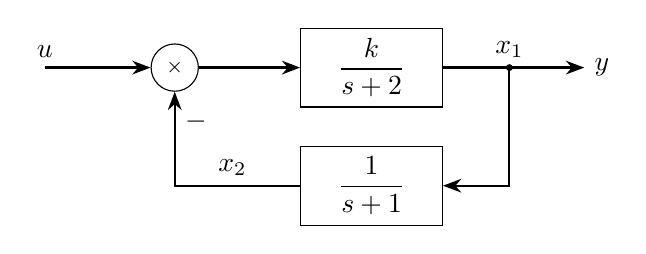
\begin{tikzpicture}[>=Stealth,
  block/.style={draw,minimum width=1.8cm,minimum height=1cm},
  add/.style={draw,circle,inner sep=0pt,minimum size=6mm}]
  \node[add] (sum) at (0,0) {$\scriptstyle\times$};
  \node[block] (plant) at (2.5,0) {$\dfrac{k}{s+2}$};
  \node[block] (sense) at (2.5,-1.5) {$\dfrac{1}{s+1}$};
  \draw[thick,->] (-1.65,0) node[above] {$u$} -- (sum.west);
  \draw[thick,->] (sum.east) -- (plant.west);
  \draw[thick,->] (plant.east) -- (5.2,0) node[right] {$y$};
  \fill (4.25,0) circle (1.25pt) node[above] {$x_1$};
  \draw[thick,->] (4.25,0) |- (sense.east);
  \draw[thick,->] (sense.west) -|
    node[pos=.27,above] {$x_2$} node[pos=.84,right] {$-$} (sum.south);
\end{tikzpicture}
\end{center}
}

\section{详细解答}

\subsection{第一步　确定求和点和各环节的输入输出}

令求和点的输出为 $e(t)$。按箭头方向，$u(t)$ 从左侧进入，返回的 $x_2(t)$ 从标有负号的端口进入，故
\[
 e(t)=u(t)-x_2(t).
\]
从前向方框出口引出的两根线具有同一信号，右边读取 $y$，下边送入反馈环节，故 $x_1(t)=y(t)$。反馈环节的出口位于方框左边，其信号是 $x_2(t)$。因此各方框的对应关系为
\[
\begin{array}{c|c|c}
\text{环节}&\text{输入}&\text{输出}\\ \hline
k/(s+2)&e&x_1\\
1/(s+1)&x_1&x_2
\end{array}
\]

\subsection{第二步　对每个方框列一阶状态方程}

一阶方框 $Z(s)/V(s)=b/(s+a)$ 表示其零状态输入输出关系。交叉相乘得 $(s+a)Z=bV$，对应 $\dot z+az=bv$。建立模型后，$z(0)$ 可单独赋值。带初值验证时，
\[
 (s+a)Z(s)=bV(s)+z(0)
\]
正是对该微分方程取单边拉普拉斯变换的结果。

前向方框给出 $(s+2)X_1=kE$，故 $\dot x_1+2x_1=ke$。反馈方框给出 $(s+1)X_2=X_1$，故 $\dot x_2+x_2=x_1$。将 $e=u-x_2$ 代入，按状态编号排列得
\[
\begin{aligned}
 \dot x_1&=-2x_1-kx_2+ku,\\
 \dot x_2&=x_1-x_2+0u,\\
 y&=x_1+0x_2+0u.
\end{aligned}
\]
$-kx_2$ 来自求和点负端信号经前向增益 $k$，而 $+x_1$ 来自反馈方框的正增益 $1$。两个符号分别由各自支路决定。

\subsection{第三步　按行读出四个矩阵}

固定 $x=[x_1,x_2]^{\mathsf T}$。$\dot x_1$ 中两状态系数为 $(-2,-k)$，输入系数为 $k$。$\dot x_2$ 中相应系数为 $(1,-1)$ 和 $0$。输出取前向方框的出口，故 $C=[1,0]$。输出没有从 $u$ 直接引入的瞬时项，所以 $D=0$。答案为
\[
 \boxed{\begin{aligned}
 \dot x&=\begin{bmatrix}-2&-k\\1&-1\end{bmatrix}x+
            \begin{bmatrix}k\\0\end{bmatrix}u,\\
 y&=\begin{bmatrix}1&0\end{bmatrix}x,\qquad D=0.
 \end{aligned}}
\]
该系统为单输入单输出，$A,B,C,D$ 的尺寸依次为 $2\times2$、$2\times1$、$1\times2$ 和 $1\times1$。

\subsection{第四步　交叉检查反馈符号}

\textbf{由原框图检查。} 零初值时
\[
Y=\frac{k}{s+2}(U-X_2),\qquad X_2=\frac{Y}{s+1}.
\]
把第二式代入第一式，并把包含 $Y$ 的量移到左边，得到
\[
 \frac{Y}{U}=\frac{k(s+1)}{(s+2)(s+1)+k}.
\]
框图的反馈负号在移项后变成分母中的 $+k$。如果算出 $-k$，应重新检查求和点与 $A_{12}$。

\textbf{由状态方程检查。} 有
\[
 sI-A=\begin{bmatrix}s+2&k\\-1&s+1\end{bmatrix},\qquad
 (sI-A)^{-1}B
 =\frac{1}{(s+2)(s+1)+k}
  \begin{bmatrix}s+1&-k\\1&s+2\end{bmatrix}\!
  \begin{bmatrix}k\\0\end{bmatrix}
 =\frac{\begin{bmatrix}k(s+1)\\k\end{bmatrix}}{(s+2)(s+1)+k}.
\]
左乘 $C$ 后取第一分量，与从原框图求得的式子一致。$k=0$ 时 $B=0$，外部输入不产生零状态输出，但有初值时仍可能有 $y(t)=x_1(0)\mathrm e^{-2t}$。

\section{同类题怎么做}

\subsection{从方框读到矩阵}

\begin{enumerate}
 \item 固定题设状态次序，为每个求和点写一个带符号的代数式。
 \item 对每个一阶方框 $b/(s+a)$ 写 $\dot z=-az+bv$，其中 $v$ 为该方框的输入，$z$ 为该方框的输出。
 \item 消去中间信号，按 $\dot x_1,\dot x_2,\ldots$ 写 $A,B$ 的各行，再沿 $y$ 的取样位置写 $C,D$。
 \item 从闭环框图独立算一次 $Y/U$，与 $C(sI-A)^{-1}B+D$ 比较。反馈支路本身有增益时，要同时核对反馈符号和两个方框增益所在的矩阵元素。
\end{enumerate}

\subsection{变式　回授改为正反馈或改变支路增益}

考虑前向环节 $g/(s+p)$、回授环节 $h/(s+q)$。仍取两方框输出为 $x_1,x_2$，并令求和点为 $u+\sigma x_2$，其中 $\sigma=-1$ 表示负反馈，$\sigma=1$ 表示正反馈。则
\[
 A=\begin{bmatrix}-p&\sigma g\\h&-q\end{bmatrix},\quad
 B=\begin{bmatrix}g\\0\end{bmatrix},\quad C=[1,0],\quad D=0,\qquad
 G(s)=\frac{g(s+q)}{(s+p)(s+q)-\sigma gh}.
\]
例如取 $p=2,q=1,g=3,h=2$ 并改为正反馈，便有
\[
 A=\begin{bmatrix}-2&3\\2&-1\end{bmatrix},\qquad
 \det(sI-A)=(s+2)(s+1)-6=(s+4)(s-1).
\]
如果仍用负反馈，同一组增益给出 $\det(sI-A)=s^2+3s+8$。交叉项 $\sigma g$ 和闭环常数项的变化都可以从求和点直接预判。

\subsection{延伸　只观察输出时哪些状态能看见}

回到原题，能控矩阵和能观矩阵分别为
\[
 \mathcal C=[B,AB]=\begin{bmatrix}k&-2k\\0&k\end{bmatrix},\qquad
 \mathcal O=\begin{bmatrix}C\\CA\end{bmatrix}=\begin{bmatrix}1&0\\-2&-k\end{bmatrix}.
\]
$k\ne0$ 时两个矩阵都满秩，二阶实现是最小的。$k=0$ 时两个状态均不能被输入驱动，且初始 $x_2$ 的变化不影响 $y$。若追加问内部渐近稳定范围，由
$p_A(s)=s^2+3s+(2+k)$ 可知 $k>-2$ 时两根都在开左半平面。$k=-2$ 时有一个零根，$k<-2$ 时常数项为负，存在一个正实根。

\chapter{纸质练习二：齐次状态方程的对角化}

\section{原题}

\ex{化为对角规范型并求初值响应}{
已知系统的齐次状态方程
\[
 \dot x=Ax,\qquad
 A=\begin{bmatrix}
 1&-1&0\\
 -1&1&0\\
 0&0&1
 \end{bmatrix}.
\]
通过线性变换将该系统化为对角规范型，并求方程在初始条件 $x(0)=[1,\ 1,\ 1]^{\mathsf T}$ 下的解。
}

\section{详细解答}

\subsection{第一步　求特征值}

按 $\lambda I-A$ 的第三行展开，因其前两项为零，只需计算左上二阶子式：
\[
\begin{aligned}
 \det(\lambda I-A)
 &=\begin{vmatrix}\lambda-1&1&0\\1&\lambda-1&0\\0&0&\lambda-1\end{vmatrix}\\
 &=(\lambda-1)\big[(\lambda-1)^2-1\big]
 =(\lambda-1)\lambda(\lambda-2).
\end{aligned}
\]
按 $\lambda=0,1,2$ 排列。三根互异，每根可取一条非零特征向量，这三条向量线性无关。

\subsection{第二步　逐根求特征向量}

令 $v=(v_1,v_2,v_3)^{\mathsf T}$，由 $(A-\lambda I)v=0$ 得
\[
 (1-\lambda)v_1-v_2=0,\quad
 -v_1+(1-\lambda)v_2=0,\quad
 (1-\lambda)v_3=0.
\]
分别代入三个根，保留一个自由分量：
\[
\begin{array}{c|l|c}
\lambda&\text{化简后的条件}&\text{所取向量}\\ \hline
0&v_2=v_1,\quad v_3=0 & p_0=[1,1,0]^{\mathsf T}\\[1pt]
1&v_1=0,\quad v_2=0,\quad v_3\text{ 自由} & p_1=[0,0,1]^{\mathsf T}\\[1pt]
2&v_2=-v_1,\quad v_3=0 & p_2=[1,-1,0]^{\mathsf T}
\end{array}
\]
例如在 $\lambda=2$ 处，前两式均化为 $v_1+v_2=0$，取 $v_1=1$ 即可。代回原矩阵，可直接检查 $Ap_0=0$、$Ap_1=p_1$、$Ap_2=2p_2$。

\subsection{第三步　构造变换矩阵并手算逆矩阵}

把特征向量按 $0,1,2$ 排为列，取 $x=Pz$：
\[
 P=[p_0,p_1,p_2]=\begin{bmatrix}1&0&1\\1&0&-1\\0&1&0\end{bmatrix},
 \qquad \det P=2.
\]
从 $x=Pz$ 的三个分量读出
\[
 x_1=z_1+z_3,\qquad x_2=z_1-z_3,\qquad x_3=z_2.
\]
将头两式相加与相减，并保留 $z_2=x_3$，得
\[
 z_1=\frac{x_1+x_2}{2},\qquad
 z_2=x_3,\qquad
 z_3=\frac{x_1-x_2}{2},\qquad
 P^{-1}=\begin{bmatrix}1/2&1/2&0\\0&0&1\\1/2&-1/2&0\end{bmatrix}.
\]
$P$ 是常矩阵，所以 $\dot x=P\dot z$。由 $AP=[0,p_1,2p_2]$，有 $AP=P\,\operatorname{diag}(0,1,2)$，从而
\[
 \boxed{\dot z=P^{-1}APz=\begin{bmatrix}0&0&0\\0&1&0\\0&0&2\end{bmatrix}z.}
\]
右端三行分别表示 $\dot z_1=0$、$\dot z_2=z_2$、$\dot z_3=2z_3$。

\subsection{第四步　转换初值、解三个标量方程并换回去}

先将原坐标初值转换到新坐标：
\[
 z(0)=\begin{bmatrix}
 \frac12(1+1)\\1\\\frac12(1-1)
 \end{bmatrix}=\begin{bmatrix}1\\1\\0\end{bmatrix}.
\]
标量方程 $\dot z_i=\lambda_i z_i$ 的解为 $z_i(0)\mathrm e^{\lambda_i t}$。本题因 $z_3(0)=0$，对应 $\lambda=2$ 的第三个分量保持为零。于是
\[
 z(t)=\begin{bmatrix}1\\\mathrm e^t\\0\end{bmatrix},\qquad
 \boxed{x(t)=Pz(t)=\begin{bmatrix}1\\1\\\mathrm e^t\end{bmatrix}.}
\]
直接检验有 $x(0)=[1,1,1]^{\mathsf T}$，且 $Ax(t)=[1-1,-1+1,\mathrm e^t]^{\mathsf T}=\dot x(t)$。

\subsection{第五步　写出原坐标的一般状态转移矩阵}

对任意原坐标初值 $x(0)$，先乘 $P^{-1}$，再由各模态的指数传递，最后乘 $P$。因此
\[
\begin{aligned}
 \Phi(t)
 &=P\,\operatorname{diag}(1,\mathrm e^t,\mathrm e^{2t})\,P^{-1}\\
 &=\begin{bmatrix}1&0&\mathrm e^{2t}\\1&0&-\mathrm e^{2t}\\0&\mathrm e^t&0\end{bmatrix}
   \begin{bmatrix}1/2&1/2&0\\0&0&1\\1/2&-1/2&0\end{bmatrix}\\
 &=\begin{bmatrix}
 (1+\mathrm e^{2t})/2&(1-\mathrm e^{2t})/2&0\\
 (1-\mathrm e^{2t})/2&(1+\mathrm e^{2t})/2&0\\
 0&0&\mathrm e^t
 \end{bmatrix}.
\end{aligned}
\]
例如第 $(1,2)$ 元是 $1\cdot(1/2)+\mathrm e^{2t}(-1/2)$，因此两项之间为减号。代 $t=0$ 得 $\Phi(0)=I$，对各元求导再代 $t=0$ 得 $\dot\Phi(0)=A$。任选初始时刻 $t_0$ 时，解为 $x(t)=\Phi(t-t_0)x(t_0)$。

\section{同类题怎么做}

\subsection{按特征向量解齐次状态方程}

\begin{enumerate}
 \item 求 $\det(\lambda I-A)=0$。看到分块三角结构时，先分别算对角块的特征因子。
 \item 对每个 $\lambda$ 解 $(A-\lambda I)p=0$。对重根，算 $n-\rank(A-\lambda I)$ 与该根的代数重数进行比较。
 \item 有完整特征向量组时，取 $P=[p_1,\ldots,p_n]$，让 $\Lambda$ 的根顺序与 $P$ 的列对应。用 $AP=P\Lambda$ 核对。
 \item 取 $x=Pz$，计算初始分量 $z(t_0)=P^{-1}x(t_0)$。给每个分量乘 $\mathrm e^{\lambda_i(t-t_0)}$，再换回原坐标。
\end{enumerate}

\nt{\textbf{易错}\quad $\mathrm e^{\Lambda t}$ 在模态坐标中使用，原坐标的状态转移矩阵是 $P\mathrm e^{\Lambda t}P^{-1}$。实矩阵要在实数域对角化，需要有 $n$ 个实线性无关的特征向量。}

\subsection{变式　初值激发了差模态}

保持原题矩阵，改取初值 $x(0)=[2,0,-1]^{\mathsf T}$。按手算逆变换，
\[
 z(0)=\begin{bmatrix}(2+0)/2\\-1\\(2-0)/2\end{bmatrix}
 =\begin{bmatrix}1\\-1\\1\end{bmatrix}.
\]
此时第三模态系数为 $1$，于是
\[
 z(t)=\begin{bmatrix}1\\-\mathrm e^t\\\mathrm e^{2t}\end{bmatrix},
 \qquad
 x(t)=\begin{bmatrix}1+\mathrm e^{2t}\\1-\mathrm e^{2t}\\-\mathrm e^t\end{bmatrix}.
\]
对于原题这类交换对称矩阵，也可直接把前两行相加和相减。$x_1+x_2$ 满足导数为零，$x_1-x_2$ 满足 $\frac{\mathrm d}{\mathrm dt}(x_1-x_2)=2(x_1-x_2)$，可用来核对两个模态。原初值 $x_1(0)=x_2(0)$，所以只有上述差模态消失。

\subsection{变式　重根时检查能否对角化}

若 $A=\operatorname{diag}(1,1,2)$，重根 $1$ 有两个独立特征向量，可以对角化。若矩阵改为
\[
 A=\begin{bmatrix}1&1\\0&1\end{bmatrix},
\]
则 $\det(\lambda I-A)=(\lambda-1)^2$，但 $(A-I)v=0$ 只给出 $v_2=0$，特征空间仅一维。此时用 $A=I+N$、$N^2=0$ 计算
\[
 \mathrm e^{At}=\mathrm e^t(I+tN)=\mathrm e^t\begin{bmatrix}1&t\\0&1\end{bmatrix}.
\]
例如 $x(0)=[0,1]^{\mathsf T}$ 给出 $x(t)=[t\mathrm e^t,\mathrm e^t]^{\mathsf T}$。重根时先核对特征空间维数，再选择对角化或约旦块。

\chapter{纸质练习三：对角实现与单位阶跃响应}

\section{原题}

\ex{由运动方程建立对角规范型并求响应}{
设系统的运动方程为
\[
 \ddot y(t)+(a+b)\dot y(t)+ab\,y(t)=\dot u(t)+c\,u(t),
\]
其中 $a,b,c$ 均为实数，$u(t)$ 为系统的输入，$y(t)$ 为系统的输出。
\begin{enumerate}
 \item 求系统对角规范型状态空间表达式。
 \item 当输入为单位阶跃 $u(t)=1(t)$ 时，求上述状态方程在零初始条件下的解。
\end{enumerate}
}

\section{详细解答}

\subsection{第一步　求传递函数并检查分母的根}

先求零状态的输入输出关系。以 $0^-$ 为初始时刻，输入和输出此前均为零。对方程取拉普拉斯变换，
\[
 \bigl(s^2+(a+b)s+ab\bigr)Y(s)=(s+c)U(s).
\]
因此
\[
 G(s)=\frac{Y(s)}{U(s)}=\frac{s+c}{(s+a)(s+b)}.
\]
分子次数比分母低，故 $D=\lim_{s\to\infty}G(s)=0$。原题右端含 $\dot u$，其影响体现为分子的 $s$ 项。判断能否用两个独立标量状态实现，要先看 $a,b$ 是否相等，以及根在约分后是否保留。

\subsection{第二步　互异根时求对角实现}

写成
\[
 \frac{s+c}{(s+a)(s+b)}
 =\frac{\alpha}{s+a}+\frac{\beta}{s+b}.
\]
两端乘 $(s+a)(s+b)$，得 $s+c=\alpha(s+b)+\beta(s+a)$。令 $s=-a$、$s=-b$，分别得到
\[
 c-a=\alpha(b-a),\qquad c-b=\beta(a-b).
\]
所以
\[
 \alpha=\frac{c-a}{b-a},\qquad \beta=\frac{c-b}{a-b}.
\]
回代时可先检查 $\alpha+\beta=1$，再检查 $b\alpha+a\beta=c$，它们分别对应分子的 $s$ 项与常数项。

让两个标量支路同时接受同一个输入 $u$，定义零初值时 $X_1/U=1/(s+a)$、$X_2/U=1/(s+b)$。交叉相乘后分别对应
\[
 \dot x_1=-ax_1+u,\qquad \dot x_2=-bx_2+u,\qquad
 y=\alpha x_1+\beta x_2.
\]
因此第一问在 $a\ne b$ 时的一个对角实现是
\[
 \boxed{
 A=\begin{bmatrix}-a&0\\0&-b\end{bmatrix},\quad
 B=\begin{bmatrix}1\\1\end{bmatrix},\quad
 C=\begin{bmatrix}\dfrac{c-a}{b-a}&\dfrac{c-b}{a-b}\end{bmatrix},\quad D=0.
 }
\]
取 $B=[1,1]^{\mathsf T}$ 时，两支路的留数全部放在 $C$。因为
\[
 C(sI-A)^{-1}B+D
   =[\alpha,\beta]
     \begin{bmatrix}1/(s+a)&0\\0&1/(s+b)\end{bmatrix}
     \begin{bmatrix}1\\1\end{bmatrix}
   =\frac{\alpha}{s+a}+\frac{\beta}{s+b},
\]
所以它确实复现题设传递函数。

\subsection{第三步　逐分量求零初值的阶跃响应}

由对角矩阵 $A$ 得
\[
 \Phi(t)=\mathrm e^{At}=\begin{bmatrix}\mathrm e^{-at}&0\\0&\mathrm e^{-bt}\end{bmatrix}.
\]
因为 $x(0)=0$，且对 $t>0$ 有 $u(t)=1$，只剩下输入积分：
\[
\begin{aligned}
 x(t)
 &=\int_0^t\Phi(t-\tau)B\,\mathrm d\tau
 =\int_0^t\begin{bmatrix}\mathrm e^{-a(t-\tau)}\\
                            \mathrm e^{-b(t-\tau)}\end{bmatrix}\mathrm d\tau\\
 &=\begin{bmatrix}\displaystyle\int_0^t\mathrm e^{-a\sigma}\,\mathrm d\sigma\\
                    \displaystyle\int_0^t\mathrm e^{-b\sigma}\,\mathrm d\sigma\end{bmatrix}
 \qquad(\sigma=t-\tau).
\end{aligned}
\]
换元时，$\tau=0$ 对应 $\sigma=t$，$\tau=t$ 对应 $\sigma=0$，再由 $\mathrm d\tau=-\mathrm d\sigma$ 恢复积分方向。记
\[
 F_d(t)=\int_0^t\mathrm e^{-d\sigma}\,\mathrm d\sigma
 =\begin{cases}
 \dfrac{1-\mathrm e^{-dt}}{d},& d\ne0,\\[4pt]
 t,&d=0 .
 \end{cases}
\]
第二问的状态和对应输出可以统一写成
\[
 \boxed{x(t)=\begin{bmatrix}F_a(t)\\F_b(t)\end{bmatrix},\qquad
 y(t)=\alpha F_a(t)+\beta F_b(t),\qquad t\ge0.}
\]
例如 $a=0,\ b\ne0$ 时，$x_1=t$、$x_2=(1-\mathrm e^{-bt})/b$，
\[
 y(t)=\frac{c}{b}t+\frac{b-c}{b^2}(1-\mathrm e^{-bt}).
\]
$b=0,\ a\ne0$ 时交换两支路即可。$F_d(0)=0$ 且 $F_d'=1-dF_d$ 对全部实数 $d$ 都成立，与逐行状态方程一致。若 $a,b>0$，还可用 $y(\infty)=\alpha/a+\beta/b=c/(ab)$ 核对稳态输出。

\subsection{第四步　互异根但有零极点对消}

当 $a\ne b$ 且 $c=a$ 时，$\alpha=0,\ \beta=1$，原传递函数化为 $1/(s+b)$。前面的二阶实现仍然可用，$x_1$ 有响应，但 $y=x_2=F_b(t)$。若要求最小实现，只保留 $\dot x_2=-bx_2+u$。当 $c=b$ 时，$\alpha=1,\ \beta=0$，只保留 $\dot x_1=-ax_1+u$，且 $y=F_a(t)$。

用矩阵也能检查对消。原二阶实现中
\[
 [B,AB]=\begin{bmatrix}1&-a\\1&-b\end{bmatrix},\qquad
 \begin{bmatrix}C\\CA\end{bmatrix}=
 \begin{bmatrix}\alpha&\beta\\-a\alpha&-b\beta\end{bmatrix}.
\]
两矩阵的行列式分别为 $a-b$ 和 $\alpha\beta(a-b)$。互异根时，对消前两个支路都能由输入驱动。$\alpha=0$ 或 $\beta=0$ 时，一个支路从输出中消失。

\subsection{第五步　重根时改用重极点判别}

设 $a=b=d$，直接重写分子：
\[
 G(s)=\frac{s+c}{(s+d)^2}
     =\frac{1}{s+d}+\frac{c-d}{(s+d)^2}.
\]

\textbf{若 $c=d$。} 二阶项系数为零，传递函数约成 $1/(s+d)$。可取一阶对角实现 $\dot x_1=-dx_1+u,\ y=x_1$，其阶跃解为 $x_1(t)=y(t)=F_d(t)$。若要保留两个对角状态，可取 $A=-dI_2$、$B=[1,0]^{\mathsf T}$、$C=[1,0]$、$D=0$。在零初值下 $x(t)=[F_d(t),0]^{\mathsf T}$。

这两个对角实现满足题设的零初值输入输出关系。若还要重现原二阶方程的任意初值，齐次输出可能含 $t\mathrm e^{-dt}$，应保留二阶约旦块。例如取 $\dot z_1=-dz_1+z_2+u$、$\dot z_2=-dz_2$、$y=z_1$，则 $z_2=\dot y+dy-u$，可以逐一匹配原方程给定的 $y,\dot y$ 初值。零初值时 $z_2$ 一直为零，输入只激发一阶响应。若 $z_2(0)\ne0$，则初值响应中包含 $z_2(0)t\mathrm e^{-dt}$。

\textbf{若 $c\ne d$。} 二阶极点保留，题目要求的对角实现此时不存在。对于任意有限维对角矩阵 $\operatorname{diag}(\lambda_1,\ldots,\lambda_n)$，$C(sI-A)^{-1}B+D$ 只含各项 $C_iB_i/(s-\lambda_i)$。若多个 $\lambda_i$ 相同，同分母的项相加仍只有一次因子，不能产生 $(s+d)^{-2}$。

此时取二阶约旦块，将输入加到第二个状态：
\[
 \boxed{
 A=\begin{bmatrix}-d&1\\0&-d\end{bmatrix},\quad
 B=\begin{bmatrix}0\\1\end{bmatrix},\quad C=[c-d,1],\quad D=0.
 }
\]
由 $(s+d)X_2=U$、$(s+d)X_1=X_2$ 可见 $X_2/U=(s+d)^{-1}$、$X_1/U=(s+d)^{-2}$。输出取 $y=(c-d)x_1+x_2$，与两项重极点分式逐项对应。

为求阶跃响应，将 $A=-dI+N$，其中 $N^2=0$，于是
\[
 \mathrm e^{A\sigma}=\mathrm e^{-d\sigma}
   \begin{bmatrix}1&\sigma\\0&1\end{bmatrix},\qquad
 \mathrm e^{A\sigma}B=\mathrm e^{-d\sigma}\begin{bmatrix}\sigma\\1\end{bmatrix}.
\]
记 $H_d(t)=\int_0^t\sigma\mathrm e^{-d\sigma}\,\mathrm d\sigma$。当 $d\ne0$，分部积分得
\[
 H_d(t)
 =-\frac{t}{d}\mathrm e^{-dt}+\frac{F_d(t)}{d}
 =\frac{1-(1+dt)\mathrm e^{-dt}}{d^2}.
\]
当 $d=0$ 时直接积分，得 $H_0(t)=t^2/2$。因此重极点保留时
\[
 \boxed{x(t)=\begin{bmatrix}H_d(t)\\F_d(t)\end{bmatrix},\qquad
 y(t)=(c-d)H_d(t)+F_d(t).}
\]
$F_d(0)=H_d(0)=0$，且 $\dot H_d=F_d-dH_d$，可分别核对 $\dot x_2=-dx_2+1$ 和 $\dot x_1=-dx_1+x_2$。特别地，当 $a=b=0,c\ne0$ 时，$x(t)=[t^2/2,t]^{\mathsf T}$、$y(t)=t+ct^2/2$。若此时 $c=0$，回到对消分支，$y(t)=t$。

\subsection{第六步　验算阶跃时刻与原运动方程}

单位阶跃在 $t>0$ 的普通导数为零，但在 $t=0$ 的跳变产生冲激 $\dot u=\delta(t)$。若输出 $y$ 在零时刻跳变，其二阶导数会出现 $\delta'(t)$。原方程右侧没有 $\delta'(t)$，所以 $y$ 连续。将原方程从 $0^-$ 积到 $0^+$，得到
\[
 \dot y(0^+)-\dot y(0^-)
 +(a+b)\bigl[y(0^+)-y(0^-)\bigr]=1.
\]
零历史给出 $y(0^+)=0$、$\dot y(0^+)=1$。也可在状态空间核对：$D=0$，输入是有界阶跃，$x(0^+)=0$。当 $a\ne b$ 时，$\dot y(0^+)=CB=\alpha+\beta=1$，约旦实现和一阶对消实现都给出相同结果。

对 $t>0$，方程右端等于 $c$。互异根时，$\bigl(\frac{\mathrm d}{\mathrm dt}+a\bigr)F_a=1$，再施加 $\bigl(\frac{\mathrm d}{\mathrm dt}+b\bigr)$ 得 $b$。同理，两个算子作用于 $F_b$ 得 $a$，因此作用于 $y=\alpha F_a+\beta F_b$ 的结果是 $\alpha b+\beta a=c$。若从原微分方程分段求解，应在 $t>0$ 写右端 $c$，同时使用跳变后的初值 $\dot y(0^+)=1$。

\section{同类题怎么做}

\subsection{从分式到状态响应的检查顺序}

\begin{enumerate}
 \item 先把输出最高阶系数归一化，在零历史条件下写 $Y/U$。若分子与分母同阶，先长除取 $D$，只对余下真分式分解。
 \item 分解分母，先识别对消与实际极点重数。单极点各用一个标量支路，保留的二重极点用一个二阶约旦块。
 \item 写状态积分，再左乘 $C$ 并补 $Du$。遇到零参数，把对应指数积分改成 $t$ 或 $t^2/2$。
 \item 用 $G=C(sI-A)^{-1}B+D$ 核对实现，用 $x(0^+)$、$y(0^+)$ 和右侧导数核对阶跃响应。
\end{enumerate}

\subsection{变式　分子分母同阶，输出有直联跳变}

设要求对角实现并求零状态阶跃输出，给定
\[
 G_{\rm v}(s)=\frac{2s^2+9s+8}{(s+1)(s+3)}
 =2+\frac{s+2}{(s+1)(s+3)}
 =2+\frac{1/2}{s+1}+\frac{1/2}{s+3}.
\]
长除得 $D=2$，对角实现取 $A=\operatorname{diag}(-1,-3)$、$B=[1,1]^{\mathsf T}$、$C=[1/2,1/2]$。阶跃下 $x=[F_1,F_3]^{\mathsf T}$，故
\[
 y(t)=2+\frac{1-\mathrm e^{-t}}{2}+\frac{1-\mathrm e^{-3t}}{6},
 \qquad t\ge0.
\]
这里 $x(0^+)=0$ 而 $y(0^+)=2$，跳变量来自直联项。检查直联可用 $G_{\rm v}(\infty)=2$，检查稳态可用 $G_{\rm v}(0)=8/3$。

\chapter{纸质练习四：传递矩阵的最小实现}
\label{paperwork:04}

\section{原题}

\ex{纸质练习四\quad 求传递矩阵的最小实现}{
已知
\[
    G(s)=\begin{bmatrix}
      \dfrac{s+1}{(s+2)(s+3)} & \dfrac{5s+4}{s+5}
    \end{bmatrix}.
\]
求该系统的最小实现。
}

题目来源为《纸质练习答案》第 2 页。

\nt{\textbf{所用知识点}\quad
直接传递矩阵 $D$，公共分母，能观规范 II 形，多输入通道的分子系数排列，最小阶数与实际极点。}

\section{详细解答}

\subsection{读出输入、输出和直接传递项}

$G(s)$ 有一行两列，故 $u=[u_1\ u_2]^\top$ 有两个分量，$y$ 为标量。设实现用 $n$ 个状态，
\[
    \dot x=Ax+Bu,\qquad y=Cx+Du,\qquad
    G(s)=C(sI-A)^{-1}B+D .
\]
$B$ 应有两列，$C$ 应有一行，$D$ 的尺寸固定为 $1\times2$。上式的传递矩阵从\textbf{零初态}求得。因为 $(sI-A)^{-1}$ 随 $s\to\infty$ 趋于零，逐通道取极限可得 $D=\lim_{s\to\infty}G(s)$。

第一通道的分子次数小于分母次数，它的极限为零。第二通道的分子、分母同为一次。先把分子写成分母的整数倍加余数，
\[
    5s+4=5(s+5)-21
    \quad\Longrightarrow\quad
    \frac{5s+4}{s+5}=5-\frac{21}{s+5}.
\]
因此 $D=[0\ 5]$，严格真部分为
\[
    G(s)-D=
    \begin{bmatrix}\dfrac{s+1}{(s+2)(s+3)} &-\dfrac{21}{s+5}\end{bmatrix}.
\]
时间域中，$5u_2$ 直接进入 $y$。余数 $-21$ 决定输入 $u_2$ 的动态部分，稍后进入 $B$ 的第二列。

\subsection{通分并逐次提取系数}

取公共分母 $a(s)=(s+2)(s+3)(s+5)$。先乘前两个因子，
\[
\begin{aligned}
    (s+2)(s+3)&=s^2+5s+6,\\
    a(s)&=(s^2+5s+6)(s+5)=s^3+10s^2+31s+30.
\end{aligned}
\]
第一通道分子补上 $s+5$，第二通道分子补上 $(s+2)(s+3)$，所以
\[
\begin{aligned}
    N_1(s)&=(s+1)(s+5)=s^2+6s+5,\\
    N_2(s)&=-21(s+2)(s+3)=-21s^2-105s-126 .
\end{aligned}
\]
按 $s^0,s^1,s^2$ 的顺序读取每个通道的系数，再把同一幂次的系数排在同一行。
\[
\begin{array}{c|rr}
    \text{幂次}&N_1(s)&N_2(s)\\ \hline
    s^0&5&-126\\
    s^1&6&-105\\
    s^2&1&-21
\end{array}
\qquad\Longrightarrow\qquad
    B=\begin{bmatrix}5&-126\\6&-105\\1&-21\end{bmatrix}.
\]
$B$ 的每一\textbf{列}对应一个输入通道，每一\textbf{行}对应一个分子幂次。把这三行依次记为 $r_0,r_1,r_2$，则 $G-D=(r_0+sr_1+s^2r_2)/a(s)$。

\subsection{构造能观规范 II 形}

对分母 $a(s)=s^3+a_2s^2+a_1s+a_0$，本课程的能观规范 II 形把 $-a_0,-a_1,-a_2$ 从上到下排在 $A$ 的最后一列，次对角线为 $1$，输出取最后一个状态。代入 $a_0=30,a_1=31,a_2=10$，得到
\[
 \begin{gathered}
    A=\begin{bmatrix}0&0&-30\\1&0&-31\\0&1&-10\end{bmatrix},\qquad
    B=\begin{bmatrix}5&-126\\6&-105\\1&-21\end{bmatrix},\\[-1pt]
    C=\begin{bmatrix}0&0&1\end{bmatrix},\qquad
    D=\begin{bmatrix}0&5\end{bmatrix}.
 \end{gathered}
\]
把两列输入的作用逐行写出来，便于核对符号，
\[
\boxed{\begin{aligned}
    \dot x_1&=-30x_3+5u_1-126u_2,\\
    \dot x_2&=x_1-31x_3+6u_1-105u_2,\\
    \dot x_3&=x_2-10x_3+u_1-21u_2,\\
    y&=x_3+5u_2 .
\end{aligned}}
\]

\subsection{逐通道验算传递矩阵}

完整求逆会算出许多用不到的元素。由于输出取 $x_3$，只需求行向量 $L(s)=C(sI-A)^{-1}$。设 $L=[\ell_1\ \ell_2\ \ell_3]$，用 $L(sI-A)=C$ 得
\[
    [\ell_1\ \ell_2\ \ell_3]
    \begin{bmatrix}s&0&30\\-1&s&31\\0&-1&s+10\end{bmatrix}
    =[0\ 0\ 1].
\]
比较三个分量，
\[
    s\ell_1-\ell_2=0,\qquad s\ell_2-\ell_3=0,\qquad
    30\ell_1+31\ell_2+(s+10)\ell_3=1.
\]
前两式给出 $\ell_2=s\ell_1,\ \ell_3=s^2\ell_1$。代入第三式得到
$a(s)\ell_1=1$，所以
\[
    L(s)=\frac{[1\ s\ s^2]}{a(s)}.
\]
现在分别乘 $B$ 的第一列、第二列，并加上相应的直接传递项，
\[
\begin{aligned}
    G_{11}(s)&=L(s)B_{:1}+D_{11}
     =\frac{5+6s+s^2}{a(s)}
     =\frac{(s+1)(s+5)}{(s+2)(s+3)(s+5)}
     =\frac{s+1}{(s+2)(s+3)},\\
    G_{12}(s)&=L(s)B_{:2}+D_{12}
     =\frac{-126-105s-21s^2}{a(s)}+5
     =-\frac{21}{s+5}+5
     =\frac{5s+4}{s+5}.
\end{aligned}
\]
第一行的分子出现 $s+5$ 是通分造成的，它约掉后第一通道仍是二阶。第二行的分子含 $(s+2)(s+3)$，这两个因子同样来自通分。判断整个实现的阶数时，要合并两通道各自的实际极点。

\subsection{证明阶数最小}

先作实际极点检查。第一通道在 $s=-2,-3$ 时分子分别为 $-1,-2$，所以其两个极点均保留。第二通道在 $s=-5$ 时分子为 $5(-5)+4=-21\ne0$，故它还有极点 $-5$。三个位置互异。

任意 $n$ 阶实现都满足
\[
    G(s)-D=C\frac{\operatorname{adj}(sI-A)}{\det(sI-A)}B .
\]
因此每个通道的实际极点必须是 $\det(sI-A)$ 的根。本题至少需要三个互异根，故 $n\ge3$。上述实现恰有三个状态，因而阶数已经最小。

还可用能控和能观矩阵独立验算。设 $b_1,b_2$ 是 $B$ 的两列。只需在能控矩阵 $Q_c=[B\ AB\ A^2B]$ 中找到一个三阶非零子式。取前两列与 $Ab_1$，
\[
\begin{aligned}
    Ab_1&=
    \begin{bmatrix}0&0&-30\\1&0&-31\\0&1&-10\end{bmatrix}
    \begin{bmatrix}5\\6\\1\end{bmatrix}
    =\begin{bmatrix}-30\\-26\\-4\end{bmatrix},\\
    \det[b_1\ b_2\ Ab_1]&=
    \begin{vmatrix}5&-126&-30\\6&-105&-26\\1&-21&-4\end{vmatrix}
    =5(-126)+126(2)+(-30)(-21)=252 .
\end{aligned}
\]
故 $\rank Q_c=3$。逐次右乘 $A$，得到 $CA=[0\ 1\ {-10}]$、$CA^2=[1\ {-10}\ 69]$，所以
\[
    Q_o=\begin{bmatrix}0&0&1\\0&1&-10\\1&-10&69\end{bmatrix},
    \qquad \det Q_o=-1 .
\]
实现既完全能控又完全能观，与极点下界的结论一致。

\subsection{另一种答案：用实际极点直接建模}

分解第一通道的分式，
\[
  \frac{s+1}{(s+2)(s+3)}=-\frac{1}{s+2}+\frac{2}{s+3}.
\]
例如分别乘以 $s+2$、$s+3$，再代 $s=-2$ 和 $s=-3$，便得到系数 $-1$ 和 $2$。第二通道已有 $5-21/(s+5)$。让每个极点对应一个一阶状态，取
\[
\begin{aligned}
   \dot z_1&=-2z_1+u_1,&
   \dot z_2&=-3z_2+u_1,&
   \dot z_3&=-5z_3+u_2,\\
   y&=-z_1+2z_2-21z_3+5u_2 . &&
\end{aligned}
\]
零初态下 $Z_1=U_1/(s+2)$、$Z_2=U_1/(s+3)$、$Z_3=U_2/(s+5)$，代入输出即还原 $G(s)$。这个对角实现也是三阶，所以同样是最小实现。检验维数与传递矩阵即可比较不同的答案。

\section{同类题怎么做}

\subsection{解题顺序与易错检查}

\begin{enumerate}
    \item 先数 $G(s)$ 的行与列，再对每个元素长除并约分。$D$ 的尺寸与 $G$ 相同。
    \item 从约分后的严格真部分取首一公共分母。一个输出时能观规范 II 形的初始维数等于公分母次数，一个输入时可优先用能控规范 II 形。
    \item 把公共分母系数放入 $A$，按升幂把每个分子放入 $B$ 的相应列。核对 $y=Cx+Du$ 中的直接项，最后回算每个通道。
    \item 计算能控、能观秩，或找一个能达到的状态数下界。具有多个输出的传递矩阵还可能在同一个极点需要多个独立的模态方向。
\end{enumerate}

\begin{note}
    对一般 MIMO 系统，互异极点数只是下界。例如
    $G(s)=I_2/(s+1)$ 的两个通道都只有 $-1$，但该极点的留数矩阵是 $I_2$，秩为 $2$。若只有一个状态，该留数只能写成一列乘一行，秩至多为 $1$。取 $A=-I_2,\ B=C=I_2,\ D=0$ 可用两状态实现。
\end{note}

\subsection{小变式：约分后两路输入共用一个状态}

\ex{变式\quad 两路输入共享同一个极点}{
求
\[
    \widehat G(s)=\begin{bmatrix}
        \dfrac{s+2}{(s+2)(s+3)} & \dfrac{5s+4}{s+3}
    \end{bmatrix}
\]
的最小实现。
}

\sol
第一通道先消去 $s+2$。第二通道有 $5s+4=5(s+3)-11$，所以
\[
   \widehat G(s)=[0\ 5]+\frac{[1\ {-11}]}{s+3}.
\]
共用一个状态即可，取
\[
   \dot z=-3z+u_1-11u_2,\qquad y=z+5u_2 .
\]
验算 $Z=(U_1-11U_2)/(s+3)$，得到所给 $\widehat G(s)$。其中实际极点 $-3$ 要求至少一个状态，所以该实现最小。

若沿用未约分的分母 $(s+2)(s+3)$，会得到一个二阶能观规范 II 形
\[
   \widehat A=\begin{bmatrix}0&-6\\1&-5\end{bmatrix},\quad
   \widehat B=\begin{bmatrix}2&-22\\1&-11\end{bmatrix},\quad
   \widehat C=[0\ 1],\quad\widehat D=[0\ 5].
\]
$\widehat B$ 的两列成比例，且 $\widehat A[2\ 1]^\top=[-6\ {-3}]^\top=-3[2\ 1]^\top$，故其能控秩只有 $1$。少掉的一维正是约分消去的 $-2$ 模态。本题先约分可以直接得到最低阶。

\chapter{纸质练习五：雅可比矩阵法判稳定}

\section{原题}

\ex{判断大范围渐近稳定（原题第3页）}{
试用雅可比矩阵法判断下列系统是否为大范围渐近稳定：
\[
    \dot x_1=-2x_1+x_2,\qquad
    \dot x_2=x_1-5x_2-x_2^5 .
\]
}

\nt{\textbf{本题要核对的三件事}\quad 平衡点是否唯一，雅可比矩阵的对称和是否处处负定，以及所选的李雅普诺夫函数是否径向无界。最后一项决定能否把结论推广到任意初始状态。}

\section{详细解答}

\subsection{先求出全部平衡点}

记 $f(x)=[f_1(x)\ \ f_2(x)]^{\mathsf T}$，其中
$f_1=-2x_1+x_2$、$f_2=x_1-5x_2-x_2^5$。平衡点满足
\[
    f_1=0 \ \Longrightarrow\ x_2=2x_1 \ \Longrightarrow\ x_1=\frac{x_2}{2}.
\]
代入 $f_2=0$，整理为
\[
    0=\frac{x_2}{2}-5x_2-x_2^5
      =-\frac92 x_2-x_2^5
      =-x_2\left(\frac92+x_2^4\right).
\]
括号对所有实数 $x_2$ 都严格为正，故 $x_2=0$，再得 $x_1=0$。系统只有原点一个平衡点，所以 $f(x)=0$ 当且仅当 $x=0$。

\subsection{逐项写出雅可比矩阵和对称和}

$J$ 的第 $i$ 行来自第 $i$ 条状态方程。按列对 $x_1,x_2$ 求偏导，
\[
    \frac{\partial f_1}{\partial x_1}=-2,\quad
    \frac{\partial f_1}{\partial x_2}=1,\quad
    \frac{\partial f_2}{\partial x_1}=1,\quad
    \frac{\partial f_2}{\partial x_2}=-5-5x_2^4 .
\]
于是
\[
    J(x)=\begin{bmatrix}-2&1\\1&-5-5x_2^4\end{bmatrix},\qquad
    S(x)=J(x)+J(x)^{\mathsf T}
        =\begin{bmatrix}-4&2\\2&-10-10x_2^4\end{bmatrix}.
\]
保留 $x_2$，在整个状态空间检查 $S(x)$ 的符号。二阶对称矩阵负定要求左上角为负且行列式为正。本题中
\[
    \Delta_1=-4<0,\qquad
    \Delta_2=(-4)(-10-10x_2^4)-2^2=36+40x_2^4>0 .
\]
因此每个 $x$ 处的 $S(x)$ 均严格负定。

\subsection{构造 \(V\) 并把导数算到定号}

按雅可比矩阵法取
\[
  V(x)=f(x)^{\mathsf T}f(x)
       =(-2x_1+x_2)^2+(x_1-5x_2-x_2^5)^2 .
\]
两项都是平方，且它们同时为零只可能在原点，因此 $V(0)=0$，$V(x)>0$ 对所有 $x\ne0$ 成立。

沿系统轨迹，链式法则给出 $\dot f=J(x)\dot x=J(x)f$，所以
\[
    \dot V=\dot f^{\mathsf T}f+f^{\mathsf T}\dot f
           =f^{\mathsf T}(J^{\mathsf T}+J)f
           =f^{\mathsf T}S(x)f .
\]
也可以直接乘开再配方，避免漏掉交叉项：
\[
\begin{aligned}
    \dot V
      &=-4f_1^2+4f_1f_2-(10+10x_2^4)f_2^2\\
      &=-4\left(f_1-\frac12 f_2\right)^2-(9+10x_2^4)f_2^2 .
\end{aligned}
\]
若 $\dot V=0$，第二项迫使 $f_2=0$，第一项再迫使 $f_1=0$，因此只能是 $x=0$。所以 $x\ne0$ 时 $\dot V<0$。

\subsection{补齐大范围结论：证明 \(V\) 径向无界}

两个平方里都混有 $x_1,x_2$。要证明任意方向上 $\|x\|\to\infty$ 都有 $V\to\infty$，可以先估计标量 $-x^{\mathsf T}f(x)$：
\[
\begin{aligned}
-x^{\mathsf T}f
   &=-x_1(-2x_1+x_2)-x_2(x_1-5x_2-x_2^5)\\
   &=2x_1^2-2x_1x_2+5x_2^2+x_2^6\\
   &\ge x_1^2+4x_2^2+x_2^6
    \ge x_1^2+x_2^2=\|x\|^2 .
\end{aligned}
\]
第一条不等式用了 $2x_1x_2\le x_1^2+x_2^2$。另一方面，由柯西--施瓦茨不等式，
\[
   \|x\|^2\le -x^{\mathsf T}f
          \le |x^{\mathsf T}f|
          \le \|x\|\,\|f(x)\|.
\]
对 $x\ne0$ 除以 $\|x\|$，得到 $\|f(x)\|\ge\|x\|$。在 $x=0$ 时该式也成立。因此
\[
     V(x)=\|f(x)\|^2\ge\|x\|^2
     \quad\Longrightarrow\quad
     \lim_{\|x\|\to\infty}V(x)=+\infty .
\]
任意初值的轨迹都留在由 $V(x(t_0))$ 决定的有界闭子水平集内。向量场为多项式，在有界范围内解可继续延拓。结合 $V$ 全局正定、$\dot V$ 全局负定及径向无界，得到
\[
       \boxed{\text{原点大范围渐近稳定。}}
\]

\begin{note}
只代 $x=0$ 求 $J(0)$ 的特征值，是第一法的做法，通常只能判原点附近。本题要求大范围结论，所以写的是 $J(x)$，并对任意 $x$ 检查对称和与径向无界性。
\end{note}

\section{同类题怎么做}

\subsection{先选一条能写到底的路线}

\begin{enumerate}[leftmargin=*]
    \item 令 $f(x_e)=0$。如果目标平衡点在 $x_e$，用 $z=x-x_e$ 表示离平衡点的偏差。用 $f^{\mathsf T}f$ 时，要检查在待证明的区域内它是否只在该平衡点取零值。
    \item 题目指定雅可比矩阵法时，写 $J(x)$、$S=J+J^{\mathsf T}$，计算 $V=f^{\mathsf T}f$ 和 $\dot V=f^{\mathsf T}Sf$。二阶对称矩阵用 $S_{11}<0$、$\det S>0$ 判负定。高阶对称矩阵可用顺序主子式交替变号。
    \item 要给出全局结论时，再找 $V(x)\ge c\|x\|^p$（$c,p>0$）这样的下界。如果能先得到 $-x^{\mathsf T}f(x)\ge c\|x\|^2$，就可直接推出 $\|f(x)\|\ge c\|x\|$。
    \item 若对称和只有半定，回到 $\dot V=f^{\mathsf T}Sf$ 继续检查。也可以换用 $W=\tfrac12\|x\|^2$、$x^{\mathsf T}Px$，或在 $\dot V\le0$ 时检查零导数集合的最大不变集。
\end{enumerate}

\subsection{同一原题的独立验算}

改用 $W=\frac12(x_1^2+x_2^2)$，沿轨迹有
\[
    \dot W=x_1\dot x_1+x_2\dot x_2
          =x^{\mathsf T}f(x)
          \le -\|x\|^2=-2W .
\]
因此 $\frac{d}{dt}\bigl(e^{2(t-t_0)}W(x(t))\bigr)\le0$，从而
\[
    W(x(t))\le W(x(t_0))e^{-2(t-t_0)},\qquad
    \|x(t)\|\le e^{-(t-t_0)}\|x(t_0)\| .
\]
这个二次型给出了收敛快慢的保守上界，可用来反查原题的稳定结论。原题答卷仍先写指定的雅可比矩阵法。

\subsection{把数字换成参数：什么时候能直接套？}

考虑同结构的系统
\[
    \dot x_1=-ax_1+bx_2,\qquad
    \dot x_2=bx_1-cx_2-dx_2^{2r+1},
    \qquad a,c>0,\quad d\ge0,\quad r=1,2,\ldots .
\]
其 $S=J+J^{\mathsf T}$ 的左上角为 $-2a$，行列式为
\[
    \det S(x)=4\left[ac-b^2+ad(2r+1)x_2^{2r}\right].
\]
若 $ac>b^2$，这个行列式处处为正，$S$ 处处严格负定。同时
\[
     -x^{\mathsf T}f=x^{\mathsf T}
      \begin{bmatrix}a&-b\\-b&c\end{bmatrix}x
      +d x_2^{2r+2}\ge \mu\|x\|^2 ,
\]
其中 $\mu>0$ 是该二阶对称矩阵的最小特征值。这个下界保证 $x\ne0$ 时 $f(x)\ne0$，并给出 $\|f(x)\|\ge\mu\|x\|$。于是原题的全局判定可以按同样次序写完。

若 $ac<b^2$，原点的线性化矩阵行列式为负，两个实特征值异号，故原点不稳定。$ac=b^2$ 是需要继续算的临界情况。

\subsection{临界变式：对称和半定时改算能量导数}

例如取 $a=b=c=d=1$、$r=1$：
\[
    \dot x_1=-x_1+x_2,\qquad
    \dot x_2=x_1-x_2-x_2^3 .
\]
与原题一样先算 $S$，得到 $S_{11}=-2$、$\det S=12x_2^2$。在 $x_2=0$ 上行列式为零，无法套用“$S$ 处处负定”这条条件。取 $W=\tfrac12(x_1^2+x_2^2)$ 则有
\[
\begin{aligned}
    \dot W&=x_1(-x_1+x_2)+x_2(x_1-x_2-x_2^3)\\
           &=-x_1^2+2x_1x_2-x_2^2-x_2^4
            =-(x_1-x_2)^2-x_2^4 .
\end{aligned}
\]
$\dot W=0$ 要求 $x_1=x_2$ 且 $x_2=0$，所以除原点外严格为负。$W$ 又全局正定、径向无界，故变式的原点也大范围渐近稳定。这个变式的关键是把交叉项配成平方，再用 $x_2^4$ 排除那条可能的零导数直线。

\chapter{纸质练习六：由传递函数配置状态反馈极点}

\section{原题}

\ex{纸质练习六\quad 线性状态反馈控制律}{
系统的传递函数为
\[
    G(s)=\frac{1}{s(s+4)(s+8)}.
\]
试确定线性状态反馈控制律，使闭环极点为 $-2$、$-4$、$-7$。
\par\smallskip\hfill{\footnotesize 《纸质练习答案》第 3 页}
}

\section{详细解答}

\nt{\textbf{解题顺序}\quad 选定状态并写出 $A,B,C,D$ $\to$ 检查 $(A,B)$ 的能控性 $\to$ 写 $A-BK$ $\to$ 比较两个首一多项式的同次项 $\to$ 将 $K$ 和状态定义一起写进答案。}

\subsection{从传递函数选取状态变量}

\sol 题目只给出了输入 $u$ 到输出 $y$ 的传递函数。按零初始条件写 $G(s)=Y(s)/U(s)$。先把分母展开，
\[
    (s+4)(s+8)=s^2+12s+32,\qquad
    s(s+4)(s+8)=s^3+12s^2+32s.
\]
于是
\[
    (s^3+12s^2+32s)Y(s)=U(s)
    \quad\Longrightarrow\quad
    \dddot y+12\ddot y+32\dot y=u .
\]
零初值用于传递函数与微分方程之间的转换。完成实现以后，状态方程也可以用来求任意初始状态下的响应。

题目的分子为 $1$，方程右端只有 $u$，因此可选
\[
    x=\begin{bmatrix}x_1&x_2&x_3\end{bmatrix}^{\mathsf T}
     =\begin{bmatrix}y&\dot y&\ddot y\end{bmatrix}^{\mathsf T}.
\]
按状态定义，$\dot x_1=x_2$、$\dot x_2=x_3$。由微分方程，$\dot x_3=-32x_2-12x_3+u$。合起来得到
\[
    \dot x=Ax+Bu,\qquad y=Cx+Du,
    \qquad
    A=\begin{bmatrix}0&1&0\\0&0&1\\0&-32&-12\end{bmatrix},
    \qquad B=\begin{bmatrix}0\\0\\1\end{bmatrix},
    \qquad C=\begin{bmatrix}1&0&0\end{bmatrix},\quad D=0.
\]
这里 $A$ 的最后一行按常数项、一次项、二次项的顺序，填入开环分母系数的相反数。常数项是 $0$，所以第一列底部为 $0$。也可由这组状态方程反查原题数据。零初始条件下 $X_2=sX_1$、$X_3=s^2X_1$，第三行给出 $(s^3+12s^2+32s)X_1=U$。由 $Y=X_1$ 得到题设的 $G(s)$。

\subsection{检查三个极点能否全部配置}

能控矩阵用 $B$、$AB$、$A^2B$ 作列。由于 $B=e_3$，$AB$ 直接取 $A$ 的第三列。再左乘一次 $A$，
\[
\begin{aligned}
    AB&=\begin{bmatrix}0\\1\\-12\end{bmatrix},&
    A^2B&=A\begin{bmatrix}0\\1\\-12\end{bmatrix}
         =\begin{bmatrix}1\\-12\\-32+144\end{bmatrix}
         =\begin{bmatrix}1\\-12\\112\end{bmatrix}.
\end{aligned}
\]
所以
\[
    Q_c=[B\ \ AB\ \ A^2B]
      =\begin{bmatrix}0&0&1\\0&1&-12\\1&-12&112\end{bmatrix},
    \qquad
    \det Q_c
      =1\cdot\begin{vmatrix}0&1\\1&-12\end{vmatrix}=-1 .
\]
$Q_c$ 满秩，三个状态完全能控，可以任意配置三个闭环极点。

\subsection{用负状态反馈写出闭环特征式}

取 $K=[\,k_1\ \ k_2\ \ k_3\,]$，采用 $u=v-Kx$。$v$ 是可选的外部输入，原题的镇定控制律取 $v=0$。代入状态方程可得
\[
    \dot x=Ax+B(v-Kx)=(A-BK)x+Bv .
\]
$B$ 只有第三个元素非零，故 $BK$ 只改变 $A$ 的第三行，
\[
    BK=\begin{bmatrix}0&0&0\\0&0&0\\k_1&k_2&k_3\end{bmatrix},\qquad
    A_{\mathrm{cl}}=A-BK
       =\begin{bmatrix}0&1&0\\0&0&1\\-k_1&-32-k_2&-12-k_3\end{bmatrix}.
\]
闭环极点是 $A_{\mathrm{cl}}$ 的特征值。把 $sI-A_{\mathrm{cl}}$ 的符号写全，再沿第一行展开，
\[
\begin{aligned}
    p_{\mathrm{cl}}(s)
       &=\begin{vmatrix}
           s&-1&0\\0&s&-1\\k_1&32+k_2&s+12+k_3
         \end{vmatrix}\\
       &=s\begin{vmatrix}s&-1\\32+k_2&s+12+k_3\end{vmatrix}
           +\begin{vmatrix}0&-1\\k_1&s+12+k_3\end{vmatrix}\\
       &=s\bigl[s(s+12+k_3)+(32+k_2)\bigr]+k_1\\
       &=s^3+(12+k_3)s^2+(32+k_2)s+k_1.
\end{aligned}
\]
第二个子式前的正号来自第一行第二列的元素 $-1$ 与它的代数余子式符号 $-1$ 相乘。这一步确定了常数项为 $k_1$。

\subsection{展开目标多项式并逐项求增益}

极点 $-2$、$-4$、$-7$ 分别对应因子 $s+2$、$s+4$、$s+7$，所以
\[
\begin{aligned}
    p^\ast(s)&=(s+2)(s+4)(s+7)\\
             &=(s^2+6s+8)(s+7)\\
             &=s^3+(6+7)s^2+(8+6\cdot7)s+8\cdot7\\
             &=s^3+13s^2+50s+56 .
\end{aligned}
\]
目标特征式与实际特征式均为首一三次多项式。令同次项系数相等，
\[
\begin{array}{c|c|c|c}
    \text{幂次} & p_{\mathrm{cl}}(s)\ \text{系数}
                &p^\ast(s)\ \text{系数} &\text{求出的增益}\\ \hline
    s^2&12+k_3&13&k_3=13-12=1\\
    s^1&32+k_2&50&k_2=50-32=18\\
    s^0&k_1&56&k_1=56
\end{array}
\]
若保留新输入，$u=v-56x_1-18x_2-x_3$。原题所求可写成
\[
    \boxed{K=[\,56\ \ 18\ \ 1\,],\qquad
           u=-Kx=-56y-18\dot y-\ddot y.}
\]
增益数值与这一组状态相对应。把“$x=[y\ \ \dot y\ \ \ddot y]^{\mathsf T}$”一并写出，即明确了反馈的三个量及其顺序。

\subsection{回代并独立检查特征向量}

把 $u=v-56y-18\dot y-\ddot y$ 代回原方程并移项，
\[
   \dddot y+13\ddot y+50\dot y+56y=v .
\]
对其取零初值传递函数，$Y/V=1/[(s+2)(s+4)(s+7)]$。分子是常数 $1$，三个分母因子都保留。

还可以直接验算状态矩阵。代入 $K$ 后，
\[
    A_{\mathrm{cl}}
      =\begin{bmatrix}0&1&0\\0&0&1\\-56&-50&-13\end{bmatrix}.
\]
对每个候选极点 $p$，取 $r_p=[\,1\ \ p\ \ p^2\,]^{\mathsf T}$。代入 $A_{\mathrm{cl}}r_p$，前两项为 $p,p^2$。逐个核对第三项，
\[
\begin{array}{c|rcl|r}
    p &\multicolumn{3}{c|}{-56-50p-13p^2}&p^3\\ \hline
    -2& -56+100-52  &=& -8   & -8\\
    -4& -56+200-208 &=& -64  & -64\\
    -7& -56+350-637 &=& -343 & -343
\end{array}
\]
三个非零向量分别满足 $A_{\mathrm{cl}}r_p=pr_p$。对应三个互异的特征值，三阶系统的全部闭环极点已经核对。

\section{同类题怎么做}

\subsection{选择实现、变换坐标与处理直联项}

\begin{enumerate}
    \item \textbf{给出传递函数。}先约分，再取分母首一。若严格真部分的分母为 $s^n+a_{n-1}s^{n-1}+\cdots+a_0$，可选超对角线上为 $1$、末行为 $[-a_0\ \cdots\ {-a_{n-1}}]$ 的能控伴随实现，并取 $B=e_n$。严格真部分的分子系数按 $s^0$ 至 $s^{n-1}$ 排入 $C$。本题分子是 $1$，所以这组伴随状态正好是 $y,\dot y,\ddot y$。
    \item \textbf{给出状态方程。}先查 $\operatorname{rank}Q_c$。小阶数的非规范模型可以直接展开 $\det(sI-A+BK)$。若先用 $x=Tz$ 化为伴随形，算出的是 $z$ 坐标下的 $\widetilde K$，应写回 $K=\widetilde K T^{-1}$。有可控伴随结构且 $B=\beta e_n$ 时，每项增益等于对应分母系数之差除以 $\beta$。状态矩阵采用别的结构时，应按其闭环行列式比较。
    \item \textbf{模型有直联项。}对真有理的 $G(s)$，先用多项式除法取 $D=\lim_{s\to\infty}G(s)$，余下严格真部分再做状态空间实现。对状态反馈 $u=v-Kx$，同时代入两式，
    \[
        \dot x=(A-BK)x+Bv,\qquad y=(C-DK)x+Dv .
    \]
    内部极点仍由 $A-BK$ 决定。若用 $v$ 到 $y$ 的传递函数验算，还应考虑分子与分母的约分。
\end{enumerate}

\subsection{变式：把同一对象换成非伴随状态坐标}

\ex{变式\quad 在指定的新坐标下求反馈增益}{
对象仍为 $G(s)=1/[s(s+4)(s+8)]$，规定新状态为
\[
   z_1=y,\qquad z_2=\dot y+2y,\qquad z_3=2\ddot y .
\]
以 $u=v-\widetilde K z$ 设计负状态反馈，使闭环极点仍为 $-2$、$-4$、$-7$。分别用坐标换算和闭环特征式求 $\widetilde K$。
}

\nt{\textbf{解题顺序}\quad 先把 $x$ 写成 $z$ 的线性组合 $\to$ 将原控制律换成 $z$ 坐标 $\to$ 由 $\dot z$ 重建模型 $\to$ 直接联立三个系数核对。}

\sol \textbf{用原控制律换算。}从定义反解得
$x_1=z_1$、$x_2=z_2-2z_1$、$x_3=z_3/2$，即
\[
    x=Tz,\qquad
    T=\begin{bmatrix}1&0&0\\-2&1&0\\0&0&1/2\end{bmatrix},\qquad
    \det T=\tfrac12.
\]
原控制律中的 $56x_1+18x_2+x_3$ 变为
\[
    56z_1+18(z_2-2z_1)+\tfrac12 z_3
    =20z_1+18z_2+\tfrac12 z_3 .
\]
所以 $\widetilde K=KT=[\,20\ \ 18\ \ 1/2\,]$。

\textbf{从新模型直接算。}把 $\dot z_1=x_2$、$\dot z_2=x_3+2x_2$、$\dot z_3=2(-32x_2-12x_3+u)$ 逐项改写为 $z$，
\[
    \dot z=
    \begin{bmatrix}
        -2&1&0\\-4&2&1/2\\128&-64&-12
    \end{bmatrix}z+
    \begin{bmatrix}0\\0\\2\end{bmatrix}u,\qquad
    y=\begin{bmatrix}1&0&0\end{bmatrix}z.
\]
例如，$\dot z_3=-64(z_2-2z_1)-24(z_3/2)+2u=128z_1-64z_2-12z_3+2u$。
$T$ 可逆，坐标改变保持能控矩阵的秩。令 $\widetilde K=[\,\ell_1\ \ \ell_2\ \ \ell_3\,]$，反馈使新状态矩阵的末行为 $[\,128-2\ell_1\ \ {-64-2\ell_2}\ \ {-12-2\ell_3}\,]$。新闭环特征式为
\[
\begin{aligned}
    p_z(s)
     &=\begin{vmatrix}
         s+2&-1&0\\
         4&s-2&-1/2\\
         -128+2\ell_1&64+2\ell_2&s+12+2\ell_3
       \end{vmatrix}\\
     &=(s+2)\bigl[(s-2)(s+12+2\ell_3)+32+\ell_2\bigr]\\
     &\quad +4(s+12+2\ell_3)-64+\ell_1\\
     &=s^3+(12+2\ell_3)s^2+(32+\ell_2)s+2\ell_2+\ell_1 .
\end{aligned}
\]
由 $p_z(s)=s^3+13s^2+50s+56$，依次得到
\[
    12+2\ell_3=13,\qquad
    32+\ell_2=50,\qquad
    2\ell_2+\ell_1=56.
\]
因此 $\ell_3=1/2$、$\ell_2=18$、$\ell_1=20$。将它们代回，三项系数为 $12+1=13$、$32+18=50$、$36+20=56$，极点仍为 $-2,-4,-7$。两种方法求得同一组新坐标增益。

\chapter{纸质练习七：串联系统的结构与稳定性}
\label{paperwork:07}

\section{原题}

\ex{纸质练习七\quad 串联系统的建模、能控性、能观性与稳定性}{
已知两个单输入单输出系统 $S_1,S_2$ 的状态方程和输出方程为
\[
\begin{aligned}
  S_1:\quad &\dot{\boldsymbol{x}}_1
       =\begin{bmatrix}0&1\\-3&-4\end{bmatrix}\boldsymbol{x}_1
          +\begin{bmatrix}0\\1\end{bmatrix}u_1,\qquad
          y_1=\begin{bmatrix}2&1\end{bmatrix}\boldsymbol{x}_1,\\
  S_2:\quad &\dot x_2=-2x_2+u_2,\qquad y_2=x_2 .
\end{aligned}
\]
将两系统按图所示串联，串联后的系统记为 $S$。

\begin{center}
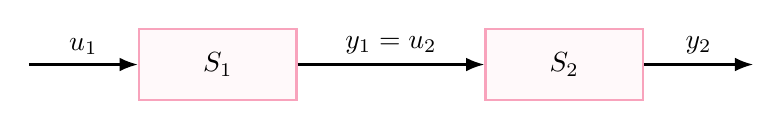
\begin{tikzpicture}[>=Latex,
 box/.style={draw=whusakura,fill=whusakura!7,thick,minimum width=2cm,minimum height=9mm}]
  \node[box] (s1) at (2.4,0) {$S_1$};
  \node[box] (s2) at (6.8,0) {$S_2$};
  \draw[->,thick] (0,0) -- node[above] {$u_1$} (s1.west);
  \draw[->,thick] (s1.east) -- node[above] {$y_1=u_2$} (s2.west);
  \draw[->,thick] (s2.east) -- node[above] {$y_2$} (9.2,0);
\end{tikzpicture}
\end{center}

\begin{enumerate}
    \item 求图示串联系统 $S$ 的状态方程和输出方程。
    \item 分析串联后系统 $S$ 的能控性和能观性。若不完全能控，作能控性分解并写出能控子系统。若不完全能观，作能观性分解并写出能观子系统。
    \item 分析系统 $S$ 在平衡态 $x_e=0$ 的渐近稳定性与系统的 BIBO 稳定性。
\end{enumerate}
}

题目及串联图来源为《纸质练习答案》第 3--4 页。

\nt{\textbf{所用知识点}\quad
串联接线与块矩阵，能控和能观的秩判据，选能控列构造状态变换，传递函数零极点相消，内部渐近稳定与 BIBO 稳定。}

\section{详细解答}

\subsection{第（1）问：按接线关系写出联合状态模型}

把 $S_1$ 的两个状态分别记为 $x_{11},x_{12}$，即 $\boldsymbol{x}_1=[x_{11}\ x_{12}]^\top$。$S_2$ 的标量状态仍记为 $x_2$。联合状态、外部输入与外部输出选为
\[
    x=[x_{11}\ x_{12}\ x_2]^\top,\qquad u=u_1,\qquad y=y_2 .
\]
串联端口满足 $u_2=y_1=2x_{11}+x_{12}$。把它代入 $\dot x_2=-2x_2+u_2$，得到
\[
\begin{cases}
    \dot x_{11}=x_{12},\\
    \dot x_{12}=-3x_{11}-4x_{12}+u,\\
    \dot x_2=2x_{11}+x_{12}-2x_2,\\
    y=x_2 .
\end{cases}
\]
前级方程不含后级状态，故 $A$ 的右上 $2\times1$ 块为零。后级从前级接收的状态组合为 $[2\ 1]\boldsymbol x_1$，故 $A$ 的左下块为 $[2\ 1]$。本题前级输出无直接输入项，外部 $u$ 只显式出现在 $\dot x_{12}$ 中。因此
\[
    \boxed{\dot x=Ax+Bu,\qquad y=Cx+Du}
\]
中的矩阵为
\[
    A=\begin{bmatrix}0&1&0\\-3&-4&0\\2&1&-2\end{bmatrix},
    \quad B=\begin{bmatrix}0\\1\\0\end{bmatrix},
    \quad C=\begin{bmatrix}0&0&1\end{bmatrix},
    \quad D=0 .
\]

\subsection{第（2）问：分别计算能控矩阵和能观矩阵}

\textbf{状态能控性。} 系统有三个状态，构造 $Q_c=[B\ AB\ A^2B]$。因为 $B=e_2$，$AB$ 就是 $A$ 的第二列。把该结果再左乘 $A$，
\[
\begin{aligned}
    AB&=\begin{bmatrix}1\\-4\\1\end{bmatrix},\\
    A^2B&=\begin{bmatrix}0&1&0\\-3&-4&0\\2&1&-2\end{bmatrix}
        \begin{bmatrix}1\\-4\\1\end{bmatrix}
      =\begin{bmatrix}-4\\-3+16\\2-4-2\end{bmatrix}
      =\begin{bmatrix}-4\\13\\-4\end{bmatrix}.
\end{aligned}
\]
并列三列，
\[
    Q_c=\begin{bmatrix}0&1&-4\\1&-4&13\\0&1&-4\end{bmatrix}.
\]
第一行与第三行相同，故秩至多为 $2$。左上二阶子式
$\begin{vmatrix}0&1\\1&-4\end{vmatrix}=-1$ 非零，故 $\rank Q_c=2<3$。也可用明确的列关系
\[
    A^2B=-3B-4AB
\]
复核。系统\textbf{不完全能控}，能控部分有两维。

\textbf{状态能观性。} $C=e_3^\top$，故 $CA$ 是 $A$ 的第三行 $[2\ 1\ {-2}]$。再右乘一次 $A$，
\[
\begin{aligned}
    CA^2 &=[2\ 1\ {-2}]
       \begin{bmatrix}0&1&0\\-3&-4&0\\2&1&-2\end{bmatrix}\\
         &=[0-3-4\quad 2-4-2\quad 4]=[-7\ {-4}\ 4].
\end{aligned}
\]
把三行叠在一起，沿第一行展开行列式，
\[
    Q_o=\begin{bmatrix}0&0&1\\2&1&-2\\-7&-4&4\end{bmatrix},
    \qquad \det Q_o=\begin{vmatrix}2&1\\-7&-4\end{vmatrix}
             =-8+7=-1 .
\]
因此 $\rank Q_o=3$，系统\textbf{完全能观}，题目要求的结构分解只需做能控性分解。

\subsection{第（2）问续：构造 $P_c$，逐块提取能控子系统}

$B,AB$ 线性无关，取它们为 $P_c$ 的前两列。第三列可取 $e_3$，它的第一分量与第三分量不同，而能控子空间内所有向量的这两个分量相同。因此三列独立，
\[
    P_c=[B\ AB\ e_3]=\begin{bmatrix}0&1&0\\1&-4&0\\0&1&1\end{bmatrix}.
\]
规定旧坐标与新坐标的关系为 $x=P_cz$。逐行读出
\[
    x_{11}=z_2,\qquad
    x_{12}=z_1-4z_2,\qquad
    x_2=z_2+z_3 .
\]
反解得 $z_1=4x_{11}+x_{12},\ z_2=x_{11},\ z_3=x_2-x_{11}$，故
\[
    P_c^{-1}=\begin{bmatrix}4&1&0\\1&0&0\\-1&0&1\end{bmatrix}.
\]
现在逐列算 $AP_c$。前两列分别是 $AB,A^2B$，第三列是 $Ae_3=-2e_3$，所以
\[
    AP_c=\begin{bmatrix}1&-4&0\\-4&13&0\\1&-4&-2\end{bmatrix}.
\]
左乘 $P_c^{-1}$ 给出新坐标中的系统矩阵。$B$ 是 $P_c$ 的第一列，所以 $P_c^{-1}B=e_1$。$C$ 取第三分量，所以 $CP_c$ 是 $P_c$ 的最后一行。完整结果为
\[
\begin{aligned}
   \bar A&=P_c^{-1}AP_c
      =\begin{bmatrix}
        4-4&-16+13&0\\1&-4&0\\-1+1&4-4&-2
      \end{bmatrix}
      =\begin{bmatrix}0&-3&0\\1&-4&0\\0&0&-2\end{bmatrix},\\
   \bar B&=P_c^{-1}B=\begin{bmatrix}1\\0\\0\end{bmatrix},
   \qquad \bar C=CP_c=[0\ 1\ 1],\qquad \bar D=0 .
\end{aligned}
\]
把前三个矩阵按前两维与最后一维分块，
\[
\begin{aligned}
    \dot z_c&=\underbrace{\begin{bmatrix}0&-3\\1&-4\end{bmatrix}}_{A_c}z_c
                   +\underbrace{\begin{bmatrix}1\\0\end{bmatrix}}_{B_c}u,
      &z_c&=[z_1\ z_2]^\top,\\
    \dot z_3&=-2z_3,\qquad
    y=\underbrace{[0\ 1]}_{C_c}z_c+z_3 .
\end{aligned}
\]
本题两块之间的动力学耦合均为零。令 $z_3$ 的初值为零并保留 $z_c$，得到能控子系统
\[
    \boxed{\dot z_c=\begin{bmatrix}0&-3\\1&-4\end{bmatrix}z_c
                          +\begin{bmatrix}1\\0\end{bmatrix}u,\qquad
            y_c=[0\ 1]z_c .}
\]
验算 $[B_c\ A_cB_c]=I_2$。其能观矩阵为
$\begin{bmatrix}0&1\\1&-4\end{bmatrix}$，行列式为 $-1$，故这个两状态实现也是最小实现。

\subsection{用原变量检查不能控坐标和初值项}

由接线后的标量方程直接相减，
\[
   \frac{\mathrm d}{\mathrm dt}(x_2-x_{11})
   =2x_{11}+x_{12}-2x_2-x_{12}=-2(x_2-x_{11}).
\]
因此无论施加什么 $u(t)$，都有
\[
    z_3(t)=e^{-2t}\bigl(x_2(0)-x_{11}(0)\bigr),\qquad
    y(t)=x_{11}(t)+e^{-2t}\bigl(x_2(0)-x_{11}(0)\bigr).
\]
初始差值决定这个模态的幅值。它进入输出，因此可被观测。零初态下该项恒为零，因此不会出现在从 $u$ 到 $y$ 的传递函数中。

例如，令 $u=0$、$x(0)=[0\ 0\ 1]^\top$，得到 $x_{11}=x_{12}=0$、$y=e^{-2t}$。这个初态实验可以在输出中看到传递函数已经约掉的 $-2$ 模态。也可以作 PBH 验算。取 $w^\top=[-1\ 0\ 1]$，则
$w^\top A=[2\ 0\ {-2}]=-2w^\top$，且 $w^\top B=0$。相应的右特征向量可取 $e_3$，因为 $Ae_3=-2e_3$ 且 $Ce_3=1$。同一模态不能控而能观。

\subsection{第（3）问：先判内部稳定，再判 BIBO 稳定}

\textbf{内部渐近稳定。} 沿 $sI-A$ 的第三列展开，
\[
\begin{aligned}
    \det(sI-A)
     &= (s+2)\begin{vmatrix}s&-1\\3&s+4\end{vmatrix}
      = (s+2)\bigl[s(s+4)+3\bigr]\\
     &= (s+2)(s+1)(s+3).
\end{aligned}
\]
特征值 $-1,-2,-3$ 都严格位于开左半平面，故零输入时任意初态都收敛到原点，$x_e=0$ 大范围渐近稳定。显式检验时，令 $u=0$，则
$\ddot x_{11}+4\dot x_{11}+3x_{11}=0$。记 $a=x_{11}(0),\ b=x_{12}(0),\ c=x_2(0)$，令
$x_{11}(t)=\alpha e^{-t}+\beta e^{-3t}$。由 $\alpha+\beta=a,\ -\alpha-3\beta=b$ 解得
\[
    x_{11}(t)=\frac{3a+b}{2}e^{-t}-\frac{a+b}{2}e^{-3t},
    \qquad x_2(t)=x_{11}(t)+(c-a)e^{-2t}.
\]
$x_{12}=\dot x_{11}$ 也趋于零。

\textbf{BIBO 稳定。} 取零初态，$S_1$ 的状态方程经拉普拉斯变换得到
\[
\begin{aligned}
   sX_{11}&=X_{12},&
   sX_{12}&=-3X_{11}-4X_{12}+U_1,\\
   X_{11}&=\frac{U_1}{s^2+4s+3},&
   Y_1&=(s+2)X_{11}.
\end{aligned}
\]
因此 $G_1(s)=(s+2)/[(s+1)(s+3)]$。$S_2$ 满足 $(s+2)X_2=U_2$ 且 $Y_2=X_2$，所以 $G_2(s)=1/(s+2)$。由 $U_2=Y_1$ 得
\[
     G_S(s)=G_2(s)G_1(s)
       =\frac{1}{s+2}\frac{s+2}{(s+1)(s+3)}
       =\frac{1}{(s+1)(s+3)}.
\]
对本题的能控子系统也可直接算出同一结果。$\dot z_2=z_1-4z_2$ 给出 $Z_1=(s+4)Z_2$，代入
$sZ_1=-3Z_2+U$ 即得 $Z_2/U=1/[s(s+4)+3]$。$-2$ 模态只影响原系统的初值响应。

约分后的极点 $-1,-3$ 均在开左半平面。进一步用冲激响应核验，
\[
    G_S(s)=\tfrac12\left(\frac1{s+1}-\frac1{s+3}\right),\qquad
    g(t)=\tfrac12(e^{-t}-e^{-3t})\quad(t\ge0).
\]
$g(t)\ge0$，且 $\int_0^\infty|g(t)|\,\mathrm dt=\frac12(1-\frac13)=\frac13$。因此对任意有界输入，零初态下
\[
    |y(t)|=\left|\int_0^t g(t-\tau)u(\tau)\,\mathrm d\tau\right|
       \le \frac13\|u\|_\infty .
\]
所以原串联系统也 BIBO 稳定。

\section{同类题怎么做}

\subsection{解题顺序与易错检查}

\begin{enumerate}
    \item 顺着箭头列端口关系。若 $u_2=y_1$ 且两个子系统都有直接项，按 $x=[x_1^\top\ x_2^\top]^\top$ 堆叠时，
    \[
       A=\begin{bmatrix}A_1&0\\B_2C_1&A_2\end{bmatrix},\quad
       B=\begin{bmatrix}B_1\\B_2D_1\end{bmatrix},\quad
       C=[D_2C_1\ C_2],\quad D=D_2D_1 .
    \]
    矩阵乘积的次序与接线方向一致。BIBO 分析对应 $G_2G_1$。
    \item 先组装再判秩。即使两个子系统各自能控、能观，串联后仍可能因相消出现隐藏模态。本题 $[B_1\ A_1B_1]$ 和 $[C_1^\top\ (C_1A_1)^\top]^\top$ 的行列式均为 $-1$，$S_2$ 的两个一阶判据均为 $1$，但联合的 $Q_c$ 只有秩 $2$。
    \item 做能控性分解时，从 $Q_c$ 取独立\textbf{列}放入 $P$ 的前几列。做能观性分解时，从 $Q_o$ 取独立\textbf{行}放入 $P^{-1}$ 的前几行。同一题里采用 $x=Pz$ 后，统一使用 $P^{-1}AP,\ P^{-1}B,\ CP$。
    \item 保留全模型判内部稳定，用最简传递函数判 BIBO 稳定。写最小实现或零初态响应时可以去掉约掉的模态，讨论任意初值时仍须保留其状态和输出贡献。
\end{enumerate}

\subsection{小变式：相消掉的模态本身不稳定}

\ex{变式\quad 把相消点移到右半平面}{
保留原题的 $S_1$ 状态方程与串联方向，将前级输出改为 $y_1=-x_{11}+x_{12}$，后级改为 $\dot x_2=x_2+u_2,\ y_2=x_2$。判断串联系统的能控性、能观性、内部渐近稳定性和 BIBO 稳定性。
}

\sol
仍用 $u=u_1,\ y=x_2$ 和相同状态顺序。代入 $u_2=-x_{11}+x_{12}$ 得
\[
   \widehat A=\begin{bmatrix}0&1&0\\-3&-4&0\\-1&1&1\end{bmatrix},
   \qquad \widehat B=e_2,\quad \widehat C=e_3^\top,\quad \widehat D=0.
\]
$\widehat A\widehat B=[1\ {-4}\ 1]^\top$，$\widehat A^2\widehat B=[-4\ 13\ {-4}]^\top$，所以 $\widehat Q_c$ 与原题相同，秩为 $2$。$\widehat C\widehat A=[-1\ 1\ 1]$，再乘一次 $\widehat A$ 得 $[-4\ {-4}\ 1]$。沿 $\widehat Q_o$ 的首行 $[0\ 0\ 1]$ 展开，
\[
    \det\widehat Q_o=\begin{vmatrix}-1&1\\-4&-4\end{vmatrix}=4+4=8 .
\]
因此状态不完全能控、完全能观。沿用 $z_3=x_2-x_{11}$，得 $\dot z_3=(x_2-x_{11}+x_{12})-x_{12}=z_3$，且 $y=x_{11}+z_3$。取 $u=0,\ x(0)=[0\ 0\ 1]^\top$，就有 $y=e^t$，因此原点不稳定。

零初态下，前级分子由 $s+2$ 改为 $s-1$，后级新极点为 $+1$，故
\[
   \widehat G_S(s)
     =\frac{1}{s-1}\frac{s-1}{(s+1)(s+3)}
     =\frac{1}{(s+1)(s+3)} .
\]
输入输出传递函数与原题相同，冲激响应仍绝对可积，所以 BIBO 稳定。这个变式的 $e^t$ 只来自不能控模态的非零初值。若只依据约分后的极点判断内部状态，就会漏掉这个模态。


\end{document}
